\documentclass[a4paper,12pt]{article}
\usepackage[utf8]{inputenc}
\usepackage[francais]{babel}
\usepackage{listings}
\usepackage{textcomp}
\usepackage[usenames,dvipsnames]{xcolor}
\usepackage{titlepic}
\usepackage{graphicx}
\usepackage{hyperref}
\usepackage{chngcntr}
\usepackage{amsmath}
\usepackage{array}
\usepackage{titlesec}
\usepackage{pdflscape}

% Configuration des liens
\hypersetup{
    colorlinks,
    citecolor=black,
    filecolor=black,
    linkcolor=black,
    urlcolor=black
}

% Configuration des blocs de code
\lstdefinelanguage{JavaScript}{
  keywords={typeof, instanceof, true, false, try, catch, function, return, null, switch, var, if, in, while, do, else, case, break},
  keywordstyle=\color{blue}\bfseries,
  ndkeywords={class, export, boolean, throw, implements, import, this},
  ndkeywordstyle=\color{darkgray}\bfseries,
  identifierstyle=\color{black},
  sensitive=false,
  comment=[l]{//},
  morecomment=[s]{/*}{*/},
  commentstyle=\color{purple}\ttfamily,
  stringstyle=\color{red}\ttfamily,
  morestring=[b]',
  morestring=[b]"
}

\lstset {
upquote=true,
columns=flexible,
stringstyle=\ttfamily,
aboveskip=\topsep,
belowskip=\topsep,
breaklines,
basicstyle=\small,
breakindent=1.5em,
showstringspaces=false,
numbers=left,
frame=shadowbox,
numberstyle=\tiny\color{gray},
rulecolor=\color{gray},
language=JavaScript,
texcl=true,
commentstyle=\color{BrickRed}
}

\setcounter{secnumdepth}{4}
\setcounter{tocdepth}{4}

\titleformat{\paragraph}
{\normalfont\normalsize\bfseries}{\theparagraph}{1em}{}
\titlespacing*{\paragraph}
{0pt}{3.25ex plus 1ex minus .2ex}{1.5ex plus .2ex}

% Réinitialisation du compteur de sections pour chaque partie
% \counterwithin*{section}{part}

% Espace entre les paragraphes
\setlength{\parskip}{10pt}

% Padding dans les tableaux
\renewcommand{\arraystretch}{1.5}

% Page de garde
\title{\textbf{\texttt{HARMONEEZER}}}
\author{\textsc{Baptiste Vannesson}}
\date{\textit{\today}}

\begin{document}
\maketitle

\begin{figure}[!h]
  \begin{center}
    
\includegraphics[scale=0.1]{logo-harmoneezer.png}
  \end{center}
\end{figure}

\begin{center}
  Réalisé à l'université de Caen Normandie dans le cadre du M2-DNR2I
  
  Encadré par Sébastien Delpic, chef de projet musique à Orange Labs
\end{center}

\newpage
\tableofcontents
\newpage
\listoffigures
\listoftables
\newpage

% ==========================================================================
% ============================== Introduction ==============================
% ==========================================================================

\part*{Introduction}

Grand art parmi les arts, la musique a toujours fait partie du patrimoine culturel de l'humanité. Divinisée dans la Grèce antique, ritualisée par les peuples primitifs, intellectualisée par les illustres penseurs du siècle des Lumières, réifiée à la gloire du consumérisme, et même numérisée par le progrès technologique, la musique est partout et résolument polymorphe. De la musique tribale au Heavy Metal, en passant par le Classique, la J-pop, le Jazz, ou encore le Raï, il est clair que l'univers du son est vaste et étonnament diversifié. Il faut dire qu'à l'instar de l'architecture, de la sculpture, de la peinture, de la danse, de la littérature et du cinéma, la musique est un vecteur de communication qui puise dans la richesse des origines ethniques.

Les nostalgiques savent que la musique accompagne l'histoire, individuelle et collective. Il n'est pas rare de plonger dans une intense rétrospection à la simple écoute d'une composition qui symbolise une époque ou évoque un événement. Les nostalgiques ont aussi bien conscience que le rapport des hommes avec la musique a profondément muté au cours des derniers siècles. Probablement influencée par la révolution industrielle et l'avènement du capitalisme en Occident, la musique est devenue un produit en sus d'être un art. Il y a donc aujourd'hui une intrication évidente entre, d'une part, l'expression artistique, et d'autre part, les lois du marché.

On peut d'ailleurs noter, au-delà de la musique elle-même, que les façons de la « consommer » ne cessent de se multiplier et de converger vers une forme d'abstraction technologique. Là encore, un lien étroit se crée entre le cœur de l'expression musicale et le monde hyperconnecté dans lequel nous vivons aujourd'hui. La génération Y, pourtant jeune, a déjà connu les vinyles, les cassettes, les CDs et les fichiers MP3. À ce rythme, bien malin est celui qui pourrait prédire jusqu'où tout cela va nous mener dans les décennies à venir...

\newpage

% ==========================================================================
% ============================== I. Contexte ===============================
% ==========================================================================

\part{Contexte}

HARMONEEZER est une application qui s'inscrit dans l'air du temps. Avant de présenter concrètement le cœur du projet, il convient donc de faire un tour d'horizon du paysage musical tel qu'il est aujourd'hui afin de bien comprendre les enjeux. Nous développerons dans cette partie quelques constats empiriques fondamentaux, puis nous analyserons l'existant pour situer précisément le projet dans son contexte.

\section{Constats empiriques}

C'est un fait, la musique contemporaine est en proie à une altération continue. Il n'est pas ici question de dièses ou de bémols, mais bien de la forme sous laquelle on la retrouve et du statut qui lui est attribué en société. De nos jours, on peut dire qu'on assiste à deux événements majeurs dans le vaste monde de la musique occidentale : la crise de l'industrie du disque et l'essor de la musique numérique.

\subsection{La crise de l'industrie du disque}

Depuis environ vingt ans, l'industrie du disque est en berne. Au cours des années 1990, au même titre que le gramophone ou la platine vinyle dans un autre temps, le lecteur CD («~Compact Disc~») était sans doute le meilleur moyen pour «~consommer~» de la musique chez soi, à côté des concerts et autres représentations artistiques. L'invention du CD était en soi une petite révolution qui permettait d'avoir un son d'une qualité nettement supérieure à la bonne vieille «~K7~», tout en conservant cette compacité rendant possible le nomadisme, contrairement au vinyle.

Le développement rapide d'Internet a cependant modifié le comportement des consommateurs. En particulier, la prolifération des réseaux peer-to-peer (P2P) au début des années 2000, incarnés par des figures emblématiques telles que Napster, KaZaA, eMule, ou encore Bittorent, a amorcé la bombe du téléchargement illégal. Le phénomène a rapidement pris de l'ampleur et le partage libre de fichiers musicaux protégés a fini par entrer dans les m\oe urs, quand bien même il représente une violation systématique du droit d'auteur. Avec le P2P, la culture de la gratuité s'est installée dans les consciences, reléguant \textit{ipso facto} le CD au rang de gadget has-been réservé aux rares collectionneurs.

\subsection{L'essor de la musique numérique}

La modernité semble donner raison à la musique dématérialisée. Aujourd'hui, on ne voit plus personne dans la rue avec le mythique Walkman de Sony, ni même d'ailleurs avec le célèbre iPod d'Apple qui a largement contribué à la démocratisation du baladeur MP3. Tout se passe maintenant sur smartphone, ce qui laisse finalement peu de place pour le CD. La musique est devenue un produit intangible, comme pourrait l'être un logiciel ; un produit soumis aux lois de l'informatique puisque tout, du stockage à la lecture, dépend désormais d'un microprocesseur.

Dans ce contexte, de nouveaux acteurs ont su tirer leur épingle du jeu en utilisant Internet comme cheval de bataille. Deezer, Spotify, iTunes, Rhapsody, Bandcamp, Last.fm, SoundCloud, ... La liste est longue et témoigne de l'intérêt, culturel et économique, que représente la musique en ligne.

\section{Étude de l'existant}

La musique connectée représente un pan entier de l'Internet. En dehors des sites de e-commerce qui vendent des CDs ou des vinyles, et qui entretiennent donc le marché de la musique « physique », nous allons surtout nous intéresser ici à ce qui maintient l'évolution de la musique dans le cap de la dématérialisation. Nous parlerons bien sûr des plateformes de téléchargement (légales), des plateformes de streaming, des webradios, des APIs ou bases de données musicales, et nous terminerons sur une partie un peu particulière concernant la production d'artistes décentralisée avec le crowdfunding.

À noter tout de même que, dans les faits, la répartition des acteurs entre ces catégories n'est pas aussi tranchée, et donc il n'est pas rare de voir certains sites ou services dans plusieurs catégories. Nous tenterons donc une répartition au mieux, afin d'avoir une vision claire du milieu, sans pour autant être exhaustif.

\subsection{Plateformes de téléchargement}

La première catégorie que nous devons ici présenter est celle regroupant les plateformes de téléchargement. Nous évoquions un peu plus haut le téléchargement illégal via des réseaux pair à pair, qui a connu un développement fulgurant au début des années 2000. Son essor a d'ailleurs été si remarquable que le terme « téléchargement » a encore aujourd'hui une connotation péjorative. Mais il est bon de rappeler que le P2P n'a rien d'illégal à la base... Partager librement des fichiers de son disque dur est même louable quand il s'agit de fichiers du domaine public, ou simplement ouverts. C'est donc bel et bien l'usage détourné du P2P, via le partage de fichiers protégés par le droit d'auteur, qui est condamnable ; pas le P2P en lui-même.

De nos jours, le P2P ne représente cependant qu'une partie du téléchargement de musique sur Internet. Il existe en effet bon nombre de plateformes (commerciales ou non) sur lesquelles il est possible d'acquérir de la musique légalement, sans violation de droits. On peut citer les plus connues, à savoir : iTunes (Apple), Amazon, Rhapsody, Google Play, ou encore Bandcamp. Le modèle économique est assez classique pour la plupart des plateformes de ce type : plutôt que de payer pour un CD physique, on paye pour un morceau ou pour un album dématérialisé, ce qui donne accès au téléchargement. On retrouve donc une relation plus traditionnelle entre l'offre et la demande. La seule différence ici est que les transactions se font sur des actifs incorporels. Les sites commerciaux proposant des morceaux en téléchargement légal ne possèdent en effet rien de tangible, si ce n'est un droit immatériel de mettre en vente des fichiers audio.

Dans un autre registre, on trouve aussi, plus rarement, des plateformes qui mettent à disposition gratuitement de la musique libre de droit. On y trouve généralement des compositions tombées dans le domaine public ou sous Creative Commons, comme c'est le cas par exemple sur Jamendo ou sur Free Music Archive.

\subsection{Plateformes de streaming}

Les plateformes de téléchargement représentent une part importante du paysage musical sur Internet. Mais il existe une autre catégorie phare, tout aussi importante : le streaming.

Le streaming fait en quelque sorte écho aux premiers balbutiements du P2P car il est difficilement contrôlable et tombe rapidement dans l'illégalité, alors que tout part initialement d'un vrai progrès technologique. Le but du streaming est de fournir un cadre permettant la lecture de contenu multimédia en flux continu. Sur le Web, ce procédé a largement été supporté par Flash, mais se voit progressivement supplanté par HTML5. Avec le streaming, il est possible d'écouter de la musique directement dans le nuage (Cloud), sans aucun téléchargement préalable ; du moins au sens traditionnel du terme... Pour lire un morceau de musique en streaming, il faut bien sûr télécharger le flux qui sera lu en temps réel par un lecteur multimédia. Lorsque le streaming a lieu au sein du navigateur, la lecture d'un flux en continu est déléguée, soit à un plug-in (cf. Flash), soit tout simplement au lecteur fourni par HTML5.

Parmi les acteurs les plus connus et reconnus en matière de streaming musical, on trouve Deezer, Spotify, Jamendo, SoundCloud, mais aussi YouTube ! Ces sites en particulier proposent tous des morceaux de musique en écoute libre, accessibles sous diverses formes : streaming simple, playlists, webradios, ... Mais tous n'ont pas forcément la même stratégie pour garder leur place dans un monde où la lutte contre la violation du droit d'auteur est particulièrement agressive. Ainsi Deezer mise par exemple sur son accord avec la SACEM (Société des Auteurs, Compositeurs et Éditeurs de Musique) et sur la rémunération des artistes, tout comme Spotify qui s'est a priori engagé auprès des auteurs en leur reversant des royalties. D'autres acteurs, comme Jamendo, misent sur des licences plus souples (Creative Commons). D'autres encore, comme SoundCloud, misent davantage sur la promotion et la collaboration dans un contexte de création artistique indépendante.

YouTube fait un peu figure d'exception. Le service est en effet, dans sa conception initiale, un site de streaming vidéo, mais il s'avère largement utilisé par les internautes comme un site de streaming musical. Les vidéos contenant uniquement un morceau de musique et la pochette d'album correspondante sont légion sur YouTube ; contrairement par exemple à Dailymotion qui semble avoir une politique de surveillance plus stricte. Or bon nombre de ces pseudo-vidéos sont en infraction du droit d'auteur car mises à disposition par des tiers ne possédant pas les droits de diffusion. Mais comme il existe encore aujourd'hui un vide, ou du moins un embrouillamini législatif sur la question du streaming, cette situation risque de persévérer encore longtemps...

\subsection{Webradios}

Prolongement naturel des plateformes de streaming traditionnelles telles que Deezer, les webradios utilisent la même technologie pour diffuser de la musique en continu sur Internet. La plupart des radios connues en dehors de la sphère numérique possèdent leur propre webradio et diffusent donc aussi leur contenu en continu sur le Web. C'est le cas par exemple pour NRJ, Fun Radio, Radio Classique, Jazz Radio, ou encore Nostalgie. 

D'autres radios, au contraire, n'existent que sur Internet et sont parfois tenues par des particuliers. Il faut dire que des services tels que Radionomy facilitent grandement la mise en place d'une radio en ligne, même sans avoir de compétences techniques. Citons notamment Radio Metal, Only Classic, ou encore Hotmix Radio. Certains grands noms de la sphère numérique, à l'instar de Last.fm, ont aussi eu leur heure de gloire grâce à leur webradio.

Contrairement au streaming traditionnel qui a clairement marqué une rupture avec la consommation usuelle de disques, la webradio a en quelque sorte renoué avec la tradition en adaptant un format déjà bien connu du grand public depuis un siècle.

\subsection{APIs et bases de données musicales}

Compte tenu de la profusion de la musique en ligne et de la prolifération sans fin des acteurs qui l'alimentent, il va de soi qu'Internet regorge de ressources pour les développeurs qui souhaitent construire des applications centrées sur la musique. La plupart des grands noms possèdent leur API, comme c'est notamment le cas pour Last.fm, Deezer ou Spotify (ce dernier possédant d'ailleurs Echo Nest, en plus de sa propre API). Citons aussi MusicBrainz, une vaste base de données répertoriant plus d'un million d'artistes avec leurs sorties respectives.

Ces outils, ouverts et documentés, permettent aux développeurs de contribuer plus encore à la notoriété des différents catalogues musicaux disponibles. Mais c'est là aussi qu'on voit à quel point la musique circule facilement et librement à l'ère du numérique, quitte à propager parfois inconsciemment la violation du droit d'auteur à une échelle autrefois inconcevable. Nous parlions précédemment des effets de la dématérialisation musicale et de sa transformation en produit de consommation courante. Mais aujourd'hui, c'est même bien plus que cela... La musique est devenu un simple flux d'octets sur un réseau mondial dont personne ne peut réellement contrôler la diffusion malgré les tentatives. Les artistes eux-mêmes n'ont qu'un maigre contrôle sur la diffusion de leur propre musique, et il n'est pas rare de voir un album fuiter sur YouTube avant même qu'il ne soit officiellemment sorti.

Comme on a pu le voir, les sites sérieux mettant de la musique à disposition des internautes ont des accords leur permettant d'exploiter légalement tout ce contenu. Mais comment surveiller l'utilisation qui en est faite par des tiers, et notamment par les développeurs, dans des applications annexes ?

\subsection{Crowdfunding musical}

Venons-en maintenant à la dernière partie situant précisément HARMONEEZER dans son contexte : le crowdfunding musical.

De manière générale, le crowdfunding appartient à ce que l'on appelle communément le « Web 2.0 », c'est-à-dire le Web social au sein duquel l'utilisateur a pris le pouvoir. Le Web 2.0 met réellement l'utilisateur au centre et valorise la dimension collaborative, ou plus globalement l'UGC (« User Generated Content »). Or parmi les différentes facettes du Web 2.0, on retrouve notamment la tendance du « crowdfunding » ; autrement dit le financement participatif.

Appliqué au cas qui nous concerne, à savoir la musique, le financement participatif permet aux internautes de devenir producteurs. Dans ce créneau spécifique, on retrouve bien sûr la plateforme française My Major Company, surtout connue pour avoir révélé des artistes comme Grégoire, Joyce Jonathan, ou encore Irma. On retrouve aussi les géants américains que sont Kickstarter ou Indiegogo. Mais quelle que soit la plateforme, le principe reste le même : les artistes s'adressent directement au public pour obtenir les fonds nécessaires à la réalisation de leurs projets.

Là encore, une telle organisation a quelque peu ébranlé la conception classique du marché musical, solidement construit autour des maisons de disques et autres labels chargés de la promotion des artistes. De nos jours les internautes ne sont plus seulement des consommateurs de musique, ce sont aussi des producteurs indépendants desquels dépend le succès ou l'échec de projets artistiques.

\newpage

% ==========================================================================
% ====================== II. Présentation du projet ========================
% ==========================================================================

\part{Présentation du projet}

Dans cette section, nous allons présenter HARMONEEZER sous un angle fonctionnel. Nous aborderons par conséquent les fonctionnalités offertes par l'application, sans entrer dans les détails techniques que nous aurons l'occasion de développer dans la dernière partie de ce rapport. Nous allons ici commencer par présenter le mix harmonique qui justifie à lui seul la réalisation de ce projet. Nous parlerons ensuite de la charte graphique, et bien entendu des fonctionnalités concrètes de l'application.

\section{Le mix harmonique}

HARMONEEZER est avant tout une application capable de créer des playlists harmoniques. Et pour en arriver là, il faut s'intéresser à une technique couramment utilisée par les DJs pour soigner les transitions entre les morceaux : le \textbf{mix harmonique}. Le principe est de choisir soigneusement les morceaux qui s'enchaînent pour qu'il y ait une progression logique dans la musique. Intuitivement, on sent bien que ce n'est pas très harmonieux de mettre un morceau rapide et joyeux juste après un morceau lent et mélancolique. Mais comment codifier tout cela ? La réponse tient en trois mots : « Roue de Camelot » (cf. Figure 1 \& Figure 2).

\subsection{Roue de Camelot}

Sur la roue de Camelot, on considère qu'il y a une harmonie entre deux morceaux quand il y a correspondance de tags. Cette correspondance s'établit par adjacence non diagonale de cases, en fonction d'un morceau de référence. Pour clarifier ce galimatias, voici un exemple : si le morceau de référence a un tag 2A, alors un deuxième morceau sera compatible s'il a un tag 2A, 1A, 3A, ou 2B. S'il a un tag 1B ou 3B (diagonale), le deuxième morceau n'est pas compatible avec le premier. \textbf{Attention, un morceau réellement compatible doit avoir un tempo similaire au morceau de référence ; en théorie, la variation doit être de 5 \% grand maximum.}

\newpage

\begin{figure}[!h]
  \begin{center}
    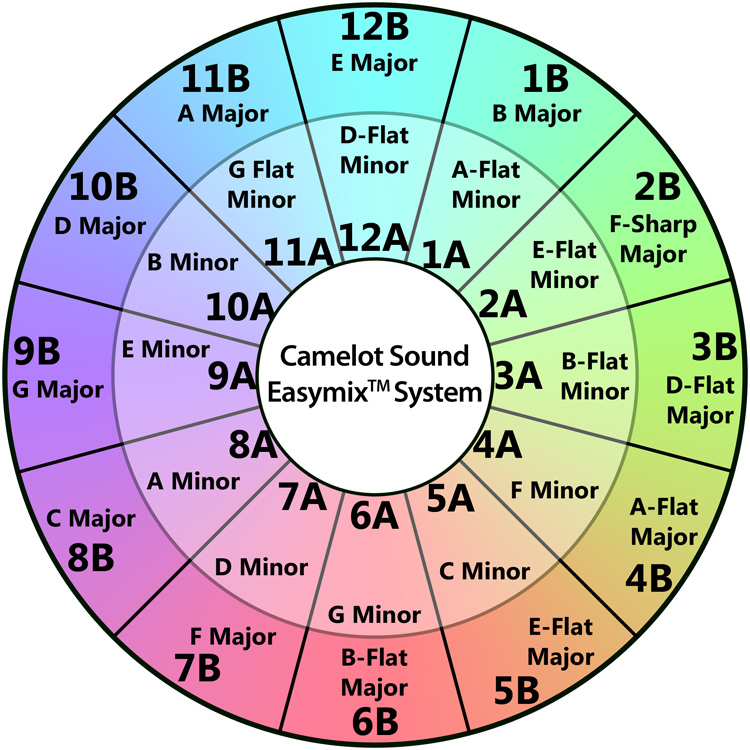
\includegraphics[scale=0.5]{camelot-wheel.jpg}
    \caption{Roue de Camelot pour le mix harmonique}
  \end{center}
\end{figure}

\newpage

\begin{figure}[!h]
  \begin{center}
    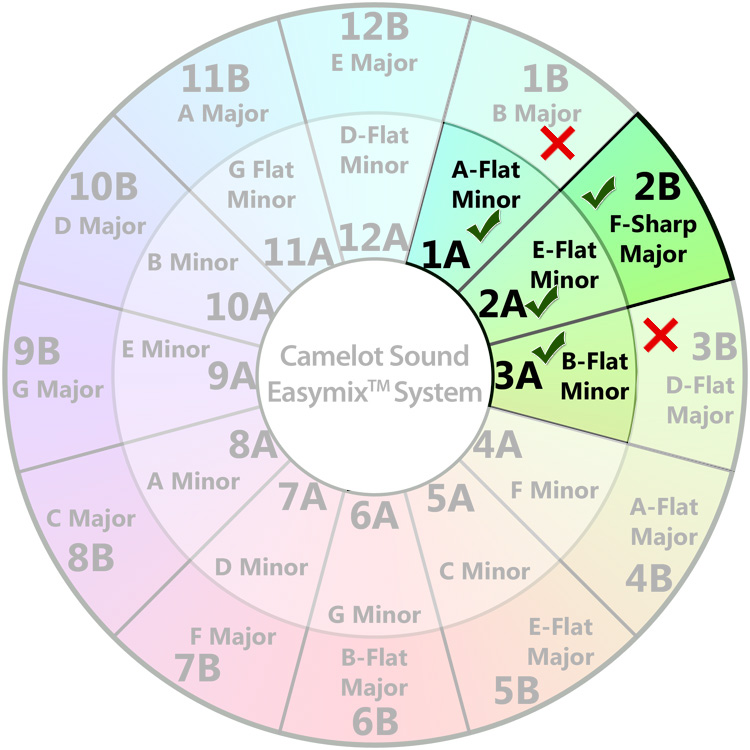
\includegraphics[scale=0.5]{camelot-wheel-harmony.jpg}
    \caption{Représentation d'une harmonie sur la Roue de Camelot}
  \end{center}
\end{figure}

\newpage

La roue de Camelot tire son origine d'un concept de théorie musicale connue sous le nom de « cycle des quintes » (ou « cercle des quartes »). Elle a été développée par Nikolay Diletsky en 1679, puis par Johann David Heinichen en 1728. C'est une théorie dans laquelle on retrouve la représentation des douze degrés de l'échelle chromatique, avec altérations et modes correspondants. La forme actuelle de la roue de Camelot provient d'un logiciel de mixage pour DJs, « Mixed In Key », qui a créé sa propre implémentation visuelle du cycle des quintes.

Pour bien comprendre ce que tout cela signifie, en particulier pour les non-musiciens, il convient d'apporter un éclairage sur quelques notions de théorie musicale qui nous concernent directement. On va donc aborder ici les notions de tempo, de degré, d'échelle chromatique, d'altérations et de modes. Le but n'est évidemment pas d'être exhaustif, mais simplement de clarifier les concepts importants pour la pleine compréhension de l'application qui s'appuie fortement sur la notion d'harmonie.

\subsection{Tempo}

Le tempo est grosso modo la vitesse d'exécution d'une composition musicale. C'est une grandeur mathématique mesurable avec un métronome, ce dernier se basant sur le nombre de pulsations ou battements par minute (BPM).

Le tempo ne doit pas être confondu avec le rythme qui détermine la durée relative des notes (rondes, blanches, noires, croches, etc.).

\subsection{Tonalité}

La tonalité est grosso modo la note (altérations et modes compris) qui caractérise un morceau de musique. Pour comprendre ce qu'est réellement la tonalité, et comment elle est représentée sur la roue de Camelot, nous devons ici présenter les notions de degrés, d'échelle chromatique, d'altérations, et de modes.

Mais avant d'aller plus loin, il est bon de donner les équivalences entre la notation alphabétique anglo-saxonne et la notation syllabique latine :

\begin{table}
  \centering
  \begin{tabular}{|c|c|}
    \hline
    Notation alphabétique & Notation syllabique \\
    \hline
    C & Do \\
    D & Ré \\
    E & Mi \\
    F & Fa \\
    G & Sol \\
    A & La \\
    B & Si \\
    \hline
  \end{tabular}
  \caption{Notations alphabétique et syllabique de la musique}
\end{table}

\newpage

De plus :

\begin{itemize}
 \item{Flat = Bémol}
 \item{Sharp = Dièse}
\end{itemize}

\subsubsection{Degrés}

En théorie musicale, un degré correspond à la position d'une note dans une échelle donnée. Il existe plusieurs échelles : pentatonique, diatonique, chromatique, etc. On parlera d'ailleurs de l'échelle chromatique après avoir présenté les degrés car c'est elle qui est utilisée dans la roue de Camelot. Mais d'abord, pour illustrer les degrés, prenons en exemple la gamme de do majeur que tout le monde connaît : do ré mi fa sol la si do. Sur une portée, on a quelque chose qui ressemble à ça :

\begin{figure}[h]
  \begin{center}
    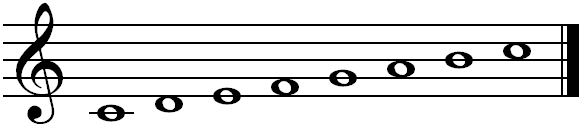
\includegraphics[scale=0.5]{gamme-do.png}
    \caption{Gamme de do majeur}
  \end{center}
\end{figure}

On utilise ici des rondes (4 temps) en guise de notes et une clé de sol pour la lecture de celles-ci sur la portée. Par définition, la note positionnée sur la deuxième ligne en partant du bas est donc un sol.
En outre, on constate que l'on a 8 notes dans la gamme ici représentée. On parle alors d'octave pour désigner l'intervalle séparant le premier do du dernier. En ajoutant la notion de degré dans cette représentation, nous avons maintenant ceci :

\begin{figure}[h]
  \begin{center}
    
\includegraphics[scale=0.4]{gamme-do-degres.png}
    \caption{Gamme de do majeur avec degrés}
  \end{center}
\end{figure}

On le voit, les notes sont ici numérotées au regard de leur position dans la gamme. Par convention, en fonction des positions (degrés), chaque note reçoit un nom spécifique.

\begin{table}[h]
  \centering
  \begin{tabular}{|c|c|}
    \hline
    \textbf{Degré} & \textbf{Nom} \\
    \hline
    I & tonique \\
    II & sus-tonique \\
    III & médiante \\
    IV & sous-dominante \\
    V & dominante \\
    VI & sus-dominante \\
    VII & sensible \\
    \hline
  \end{tabular}
  \caption{Dénomination des degrés en musique}
\end{table}

À notre niveau, on comprend donc mieux la numérotation présente sur la roue de Camelot. En fait, les numéros correspondent aux différents degrés. Mais pourquoi la roue possède-t-elle 12 degrés, et pas 7 comme nous venons de le voir ? C'est ce que nous allons expliquer en découvrant l'échelle chromatique et les altérations...

\subsubsection{Échelle chromatique \& altérations}

En musique, l'échelle chromatique est une échelle comportant 12 degrés. Cela peut paraître surprenant puisque nous ne connaissons que 7 notes (do, ré, mi, fa, sol, la, si). Mais en réalité, il existe des notes intermédiaires, obtenues par altération. Une altération est une modification qui va diminuer (bémol) ou augmenter (dièse) une note initiale d'un demi-ton.

Reprenons comme base notre gamme de do majeur. Si nous jouons toutes ses notes (à l'exception du do qui sert de conclusion) et que nous jouons de surcroît toutes les altérations possibles pour chaque note, alors nous n'avons plus seulement 7 notes, mais bien 12 : do do$\sharp$ ré ré$\sharp$ mi fa fa$\sharp$ sol sol$\sharp$ la la$\sharp$ si (do). Cela fonctionne aussi dans l'autre sens : (do) si si$\flat$ la la$\flat$ sol sol$\flat$ fa mi mi$\flat$ ré ré$\flat$ do (cf. Figure 5). On parle parfois de « gamme tempérée » pour désigner cette gamme large divisant l'octave en 12 intervalles.

\begin{figure}[h]
  \begin{center}
    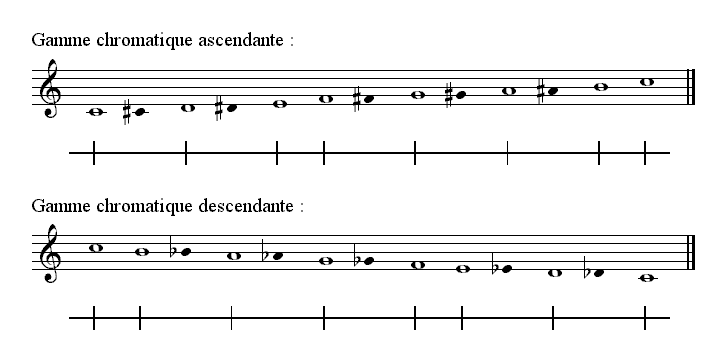
\includegraphics[scale=0.5]{gamme-chromatique.png}
    \caption{Gamme chromatique}
  \end{center}
\end{figure}

Ce qui n'est pas forcément clair ici, c'est qu'un do$\sharp$ produit exactement le même son qu'un ré$\flat$. Conceptuellement parlant, les deux existent néanmoins car le do$\sharp$ est une augmentation d'un demi-ton du do, là où le ré$\flat$ est une diminution d'un demi-ton du ré. Pour clarifier les choses, il est ainsi intéressant de visualiser comment tout cela s'organise sur un piano (cf. Figure 6).

\begin{figure}[!h]
  \begin{center}
    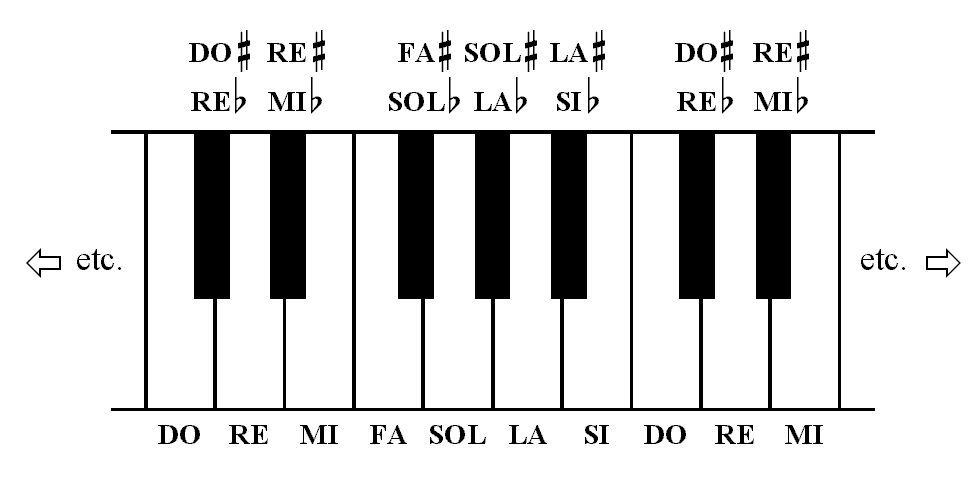
\includegraphics[scale=0.4]{clavier-piano.png}
    \caption{Visualisation des notes sur un piano}
  \end{center}
\end{figure}

À ce stade, on comprend pourquoi la roue de Camelot comporte une numérotation de 1 à 12. Il s'agit en fait des différents degrés de l'échelle chromatique, avec toutes les altérations que cela sous-entend. Ce que l'on ne comprend toujours pas, c'est la division de cette roue en deux parties. Mais c'est ce que nous allons voir maintenant avec les modes...

\newpage

\subsubsection{Modes}

Il existe deux modes principaux dans la musique occidentale : majeur et mineur. Pour certains, qui tentent de simplifier cette notion complexe, les deux modes se distingueraient par la couleur qu'ils dégagent : le mode mineur serait triste et le mode majeur joyeux. Mais de manière pragmatique, le mode majeur se distingue surtout du mode mineur par un agencement spécifique des gammes. La succession des intervalles entre degrés diffère effectivement en fonction du mode. Voici, en théorie, la structure d'une gamme majeure et la structure d'une gamme mineure :

\begin{table}[h]
  \centering
  \begin{tabular}{|c|c|c|}
    \hline
    & \textbf{Gamme majeure} & \textbf{Gamme mineure} \\
    \hline
    \textbf{Ton} & 1 1 $\frac{1}{2}$ 1 1 1 $\frac{1}{2}$ & 1 $\frac{1}{2}$ 1 1 $\frac{1}{2}$ 1 1 \\
    \hline
  \end{tabular}
  \caption{Gamme majeure et gamme mineure}
\end{table}

On comprend donc ici pourquoi la roue de Camelot est divisée en deux grandes parties. Elle prend simplement en considération les 12 degrés de l'échelle chromatique pour le mode majeur d'un côté, et pour le mode mineur d'un autre côté.

\newpage

\section{GUI \& UX}

\subsection{Modèle de navigation}

HARMONEEZER est davantage une application web qu'un site web. Cela signifie que tout est disponible sur le web et utilisable avec un simple navigateur, mais que l'utilisation générale est beaucoup moins classique qu'un défilé de pages. Dans le cas présent, nous avons une webapp monopage où tout est dynamique. L'expérience utilisateur (UX) est donc hautement interactive et personnalisée. L'utilisateur ne navigue pas ici de page en page. Il est dans un espace entièrement configurable, avec une sorte de tableau de bord, grâce auquel il peut agir et prendre des décisions qui auront une influence sur son expérience.

L'application proprement dite s'articule autour de cinq sections fondamentales, qui constituent forcément le menu :

\begin{itemize}
 \item{La playlist}
 \item{Les favoris}
 \item{Les ambiances}
 \item{Les suggestions}
 \item{La connexion de l'utilisateur}
\end{itemize}

Chacune de ces sections est matérialisée par une sidebar dans l'interface graphique, ce qui permet une grande modularité. En procédant ainsi, l'utilisateur n'est pas contraint dans sa zone de navigation, d'autant que les sidebars utlisent tout l'espace disponible en apparaissant à divers endroits de l'écran. Dans la plupart des sections, l'utilisateur se voit confronté à un certain nombre d'options. Le cas le plus typique est la section consacrée aux favoris, où tous les éléments utiles entrant dans l'utilisation de l'application sont paramétrables.

HARMONEEZER possède également une version mobile, afin que les internautes puissent y accéder depuis leur smartphone. La démarche s'appuie sur les principes du responsive design et propose donc une version allégée qui rend le service attendu, mais sans les options qui relèvent davantage d'une expérience desktop.

\subsection{Charte graphique}

Côté ergonomie, on a pris soin de maximiser les surfaces cliquables et de mettre en avant les éléments interactifs du décor. À ce titre on retrouve par exemple un iPod grandeur nature offrant quelques raccourcis utiles pour une expérience plus fun, de même qu'une barre de lecture audio faite maison interagissant avec le lecteur de Deezer.

Si l'on s'attarde maintenant sur l'aspect purement design de l'application (Graphical User Interface), on peut dire que le tout est assez contemporain et conforme à ce qui se fait sur le web dans l'industrie musicale. L'ensemble est très coloré et s'appuie sur des images en haute définition pour avoir un rendu immersif.

\section{Fonctionnalités}

HARMONEEZER est avant tout un outil permettant aux internautes de découvrir des morceaux similaires, en particulier sous l'angle harmonique. Pour servir cette mission, il se doit de proposer un certain nombre de fonctionnalités importantes, que nous allons présenter maintenant.

\subsection{Recherche et suggestion de morceaux pertinents}

La fonctionnalité de base est évidemment le moteur de recherche de morceaux. Dans un premier temps, HARMONEEZER ne renvoie pas des suggestions harmoniques pour la recherche en cours. L'application interroge d'abord Deezer avec les mots-clés entrés par l'utilisateur, puis elle fournit à ce dernier des morceaux pertinents. Ces morceaux sont présentés à l'utilisateur sous différentes formes : il y a d'un côté l'autocomplétion qui suggère les morceaux en temps réel et au format textuel, et d'un autre côté, un carousel contenant les pochettes d'albums de tous les morceaux après validation de la recherche. À ce stade, la pertinence est déterminée par Deezer, simplement en fonction de la correspondance entre ce qui est tapé par l'internaute et ce qu'il y a dans le catalogue. Il ne s'agit donc pas ici d'une quelconque similarité musicale. On essaie juste d'aiguiller la recherche avec un premier lot de suggestions.

\newpage

Lorsque l'utilisateur voit cette première liste de suggestions, il peut sélectionner un morceau en particulier qui devient de fait la référence. L'application lance alors une série de requêtes vers Deezer et Echo Nest pour récupérer toutes les informations. Le processus mis en œuvre est détaillé à la figure suivante, selon le formalisme ANSI :

\begin{figure}[!h]
  \begin{center}
    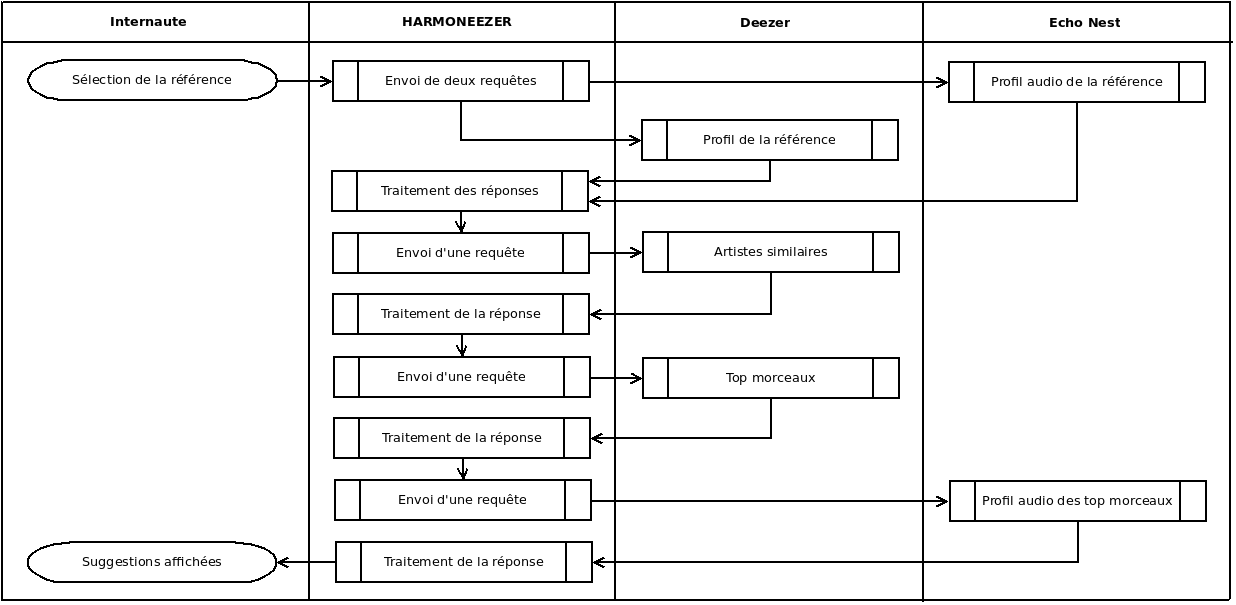
\includegraphics[scale=0.3]{processus.png}
    \caption{Processus en vigeur pour la récupération des informations}
  \end{center}
\end{figure}

À noter que Deezer recherche ici 10 artistes similaires à la référence et récupère les 5 top morceaux de chaque artiste. On a donc en théorie, à l'issue du processus de recherche, 50 morceaux potentiellement pertinents pour l'utilisateur. Mais cela est illusoire si l'on tient compte de la dimension harmonique, ce qui est bien le cas pour notre application...

En effet, pour proposer à l'utilisateur des morceaux compatibles harmoniquement avec sa recherche, il y a de nombreuses contraintes à surmonter. Tout d'abord, il faut savoir que les informations sont récupérées sur Echo Nest à partir de l'identifiant Deezer de chaque morceau. L'équivalence n'existant pas forcément entre Deezer et Echo Nest, il arrive fréquemment qu'un morceau ne soit pas trouvé sur Echo Nest. Dans le même état d'esprit, il arrive souvent qu'un morceau soit identifié sur Echo Nest mais que le résumé audio de celui-ci ne soit pas disponible ; ce qui rend impossible l'évaluation des critères sous l'angle de l'harmonie.

En règle générale, lorsque tous ces morceaux ont été éliminés de la liste finale des suggestions, il ne reste que la moitié des morceaux initialement renvoyés (soit 25 morceaux sur 50).

Au sein des morceaux qui ont été trouvés sur Echo Nest et qui possèdent bel et bien un résumé audio, il faut encore faire un tri pour savoir ceux qui sont réellement compatibles avec le morceau de référence (sous réserve que ce dernier ait un profil connu) et ceux qui ne le sont pas. L'application propose pour cela plusieurs algorithmes de tri à l'utilisateur, afin de lui laisser le choix quant à sa conception de la pertinence. Voici la liste des algorithmes disponibles :

\begin{itemize}
 \item{« Default »}
 \item{« TempoFirst »}
 \item{« KeyFirst »}
 \item{« AscendingTempo »}
 \item{« DescendingTempo »}
\end{itemize}

L'algorithme par défaut a pour objectif d'afficher en priorité les morceaux compatibles en tempo ET en tonalité, suivis des morceaux compatibles en tempo OU en tonalité, suivis des autres morceaux disponibles.

L'algorithme « TempoFirst » a pour objectif d'afficher en priorité les morceaux compatibles en tempo ET en tonalité, suivis des morceaux compatibles en tempo, suivis des morceaux compatibles en tonalité, suivis des autres morceaux disponibles.

L'algorithme « KeyFirst » a pour objectif d'afficher en priorité les morceaux compatibles en tempo ET en tonalité, suivis des morceaux compatibles en tonalité, suivis des morceaux compatibles en tempo, suivis des autres morceaux disponibles.

L'algorithme « AscendingTempo» a pour objectif d'afficher, quelle que soit la tonalité, les morceaux selon l'ordre croissant du tempo. Les morceaux les plus lents doivent donc apparaître en priorité.

L'algorithme « DescendingTempo » a pour objectif d'afficher, quelle que soit la tonalité, les morceaux selon l'ordre décroissant du tempo. Les morceaux les plus rapides doivent donc apparaître en priorité.

\subsection{Création et gestion de playlists personnalisées}

Avec HARMONEEZER, l'internaute peut créer une playlist de manière intuitive, en quelques clics seulement. Après avoir effectué une recherche et obtenu des suggestions a priori harmoniques (ou du moins similaires à la référence), l'utilisateur peut cliquer sur ce qui l'intéresse dans la liste. Le morceau est alors ajouté automatiquement dans sa playlist.

La force du système réside dans le fait que l'utilisateur peut réellement naviguer sur la roue de Camelot. En effet, à chaque fois qu'il sélectionne un morceau dans les suggestions, le morceau de référence devient le morceau cliqué et tout le processus est relancé. Ainsi on peut composer sa playlist pas à pas, avec une vraie progression harmonique !

Pour gérer une playlist, l'utilisateur a plusieurs options qui s'offrent à lui :

\begin{itemize}
 \item{Lecture aléatoire}
 \item{Lecture répétée}
 \item{Manipulation du son}
 \item{Sauvegarde de la playlist dans le navigateur}
 \item{Sauvegarde de la playlist sur son compte Deezer}
 \item{Export CSV de la playlist}
 \item{Effacement complet de la playlist}
\end{itemize}

L'utilisateur a, en outre, accès aux contrôles classiques qui lui offrent la possibilité de passer en mode lecture, en mode pause, au morceau suivant, etc. Le lecteur Flash de Deezer est utilisé ici en toile de fond, mais l'interface par défaut a été totalement repensée.

\subsection{Synchronisation d'un compte Deezer}

Pour que son expérience soit d'autant plus personnalisée, l'utilisateur a la possibilité de se connecter à l'application avec son compte Deezer. Cela lui permet notamment d'avoir un accès sans restriction aux morceaux en écoute dans sa playlist et de sauvegarder celle-ci sur son compte Deezer.

Sans cette synchronisation, l'écoute de chaque morceau est limitée à 30 secondes, et bien entendu il n'est pas possible de sauvegarder une playlist sur Deezer...

Pour que la communication entre HARMONEEZER et Deezer soit possible, il faut que l'utilisateur accorde un certain nombre de permissions à l'application lors de sa connexion. Il doit notamment autoriser l'accès à ses informations basiques sur Deezer, la gestion distante de sa bibliothèque, ainsi que la suppression d'éléments.

\subsection{Gestion des favoris}

C'est ici que l'utilisateur peut modifier le comportement par défaut de l'application s'il le souhaite. Cette section s'articule autour de trois catégories principales :

\begin{itemize}
 \item{Options diverses}
 \item{Critères de recherche}
 \item{Tri des suggestions}
\end{itemize}

Dans les options diverses, l'utilisateur peut régler un certain nombre de paramètres qui ont trait à l'ergonomie de sa navigation. En fonction de ses préférences, il est possible d'activer ou de désactiver l'iPod, les infobulles, les notifications, ou encore les sons d'ambiance.

Dans les critères de recherche, l'utilisateur peut réellement affiner ses requêtes, par exemple en réglant la tolérance qu'il souhaite accorder au tempo dans le mix harmonique. Il peut aussi activer/désactiver l'autocomplétion à la demande.

Enfin, et nous l'avons vu, l'utilisateur peut choisir l'algorithme de tri qu'il souhaite appliquer à la liste de suggestions.

\subsection{Sélection d'ambiance}

Afin que l'UX soit plus agréable et immersive, HARMONEEZER propose aux internautes de sélectionner une ambiance. Par défaut, l'ambiance est neutre ; mais voici les ambiances disponibles :

\begin{itemize}
 \item{Rock}
 \item{Electro}
 \item{Hip-Hop}
 \item{Folk}
 \item{Classique}
 \item{Jazz}
 \item{Metal}
\end{itemize}

Une ambiance se caractérise avant tout par l'image en haute définition qui tapisse le fond visuel de l'application, ainsi que par un son caractéristique lors de la sélection.

\newpage

% ==========================================================================
% ====================== III. Réalisation technique ========================
% ==========================================================================

\part{Réalisation technique}

HARMONEEZER est une application web développée intégralement en JavaScript. C'est un projet qui a donc permis d'aller beaucoup plus loin dans la compréhension de ce language et de son écosystème.

Dans le cadre de cette partie consacrée à la technique, nous commencerons par présenter l'environnement de travail, à savoir tout ce qui a été mis en place pour travailler efficacement sur le projet. Nous verrons ensuite plus en détail ce qui a été fait en matière de conception, bien que ce soit moins rigoureux que ce qu'on pourrait voir en Java par exemple, du fait de la nature même de JavaScript. Nous y reviendrons... Enfin, nous expliquerons précisément les développements effectués pour aboutir à une application fonctionnelle.

\section{Environnement de travail}

Pour travailler confortablement et efficacement, il est impératif d'avoir un environnement de travail propre et bien organisé. C'est ce que nous allons voir ici en évoquant les gestionnaires de paquets utilisés, l'intérêt du preprocessing CSS, le workflow mis en place avec un task runner, la modularisation et l'empaquetage systématique du code, et bien entendu le système de versioning.

\subsection{Gestionnaires de paquets}

En développement, lorsqu'on démarre un nouveau projet, rien n'interdit de travailler de manière un peu artisanale. L'auteur de ces lignes a souvent construit ses projets à la main, à partir de copier-coller d'autres fichiers et en allant chercher des bibliothèques à droite à gauche sur le disque ou sur Google pour récupérer les URLs des CDNs. Cette façon de faire ne pose aucun problème majeur, si ce n'est qu'elle est fastidieuse et représente un frein à la productivité. Aussi ce projet était-il une opportunité en or de se familiariser avec des outils professionnels qui permettent de gagner en efficacité.

\subsubsection{npm}

\begin{figure}[!h]
  \begin{center}
    
\includegraphics[scale=0.2]{logo-npm.png}
  \end{center}
\end{figure}

npm est le gestionnaire de paquets de Node.js. Il contient une liste astronomique de paquets utilisables par les développeurs JavaScript. Node.js étant à l'origine destiné à une utilisation en back-end, puisqu'il s'agit d'une technologie serveur, npm a été utilisé dans ce projet pour tous les modules indépendants du front-end. Cela inclut notamment les modules relatifs au serveur proprement dit, ainsi que les modules de minification, de compilation, et de validation du code source.

\textit{Toutes les dépendances sont listées dans le fichier package.json.}

\subsubsection{Bower}

\begin{figure}[!h]
  \begin{center}
    
\includegraphics[scale=0.2]{logo-bower.png}
  \end{center}
\end{figure}

Bower se présente comme étant «~un gestionnaire de paquets pour le Web~». Contrairement à npm (duquel il dépend), il est plutôt orienté front-end. Développé par Twitter, ce gestionnaire de paquets peut être utilisé conjointement avec npm. C'est notamment ce qui a été fait dans ce projet, avec une séparation claire entre les «~node\_modules~» et les «~bower\_components~». À ce titre, Bower a été logiquement utilisé pour télécharger et intégrer des bibliothèques purement front-end comme jQuery ou Vue.js.

\textit{Toutes les dépendances sont listées dans le fichier bower.json.}

\newpage

\subsection{Preprocessing CSS}

\begin{figure}[!h]
  \begin{center}
    
\includegraphics[scale=0.2]{logo-sass.png}
  \end{center}
\end{figure}

Dans la plupart des applications front-end un tant soit peu ambitieuses, et même lorsqu'un framework comme Bootstrap, Foundation ou Semantic UI est utilisé, il n'est pas rare d'avoir des fichiers CSS assez volumineux. À long terme, la maintenance de ces feuilles de style n'est pas une tâche facile, même quand elles sont soigneusement organisées. En effet, le langage CSS, bien que simple à écrire et à comprendre, n'offre pas de vrais mécanismes de factorisation de code. On a donc souvent tendance à se répéter, d'autant plus que l'architecture d'une feuille de style est plate et linéaire. C'est là qu'interviennent les préprocesseurs CSS tels que Sass, LESS, ou encore Stylus...

Dans le cadre de ce projet, le choix technologique s'est porté sur Sass, un préprocesseur écrit en Ruby qui s'avère très populaire auprès des intégrateurs. Combiné avec Compass et la syntaxe SCSS, très intuitive, Sass devient un outil puissant au service de la productivité. L'imbrication des sélecteurs CSS devient possible, permettant ainsi de créer une vraie hiérarchie au sein des feuilles de style. L'utilisation de variables et de mixins apporte en outre une flexibilité inouïe grâce à la factorisation avancée qu'elle permet.

Voici un petit condensé de la puissance de Sass avec un exemple bateau :

\begin{lstlisting}
$red: #F04A3C;

@mixin full-color($color) {
  color: $color;
  background-color: $color;
  border-color: $color;
}

#id {  
  &:hover {
    @include full-color($red);
  }
}
\end{lstlisting}

\newpage

\subsection{Workflow avec task runner}

\begin{figure}[!h]
  \begin{center}
    
\includegraphics[scale=0.2]{logo-gulp.png}
  \end{center}
\end{figure}

Lorsqu'on développe une application, quel que soit le langage, on se rend compte qu'on a souvent tendance à répéter encore et encore certaines opérations... C'est le cas par exemple pour les tâches de compilation, de validation, ou encore de minification. En partant du principe que la répétition est une mauvaise pratique en informatique (DRY - Don't Repeat Yourself), c'est vraisemblablement judicieux d'automatiser ce qui peut l'être.

Pour ce faire, JavaScript met à notre disposition des task runners, dont les plus connus sont Grunt et Gulp. Gulp étant moins verbeux et plus rapide que Grunt, c'est Gulp qui a été retenu pour ce projet.

Gulp est un outil performant qui permet réellement de gagner en efficacité. En définissant une tâche, et à l'aide de quelques lignes de JavaScript, le développeur n'a plus qu'à écrire une commande simple dans un terminal pour lancer une opération complexe. Il peut même créer des dépendances entre les tâches, afin de lancer une série d'opérations successives.

Voyons un exemple simple :

\begin{lstlisting}
// Pour utiliser Gulp, il faut d'abord importer le module
var gulp = require('gulp');

// On définit ici une tâche qui répondra au mot-clé «~hello~»
gulp.task('hello', function() {
  // On lance ce traitement lorsque la tâche a été appelée
  console.log("Hello World!");
});
\end{lstlisting}

Après avoir défini cette tâche dans gulpfile.js, le développeur n'a plus qu'à lancer «~gulp hello~» dans un terminal pour lancer le traitement, et en l'occurrence afficher «~Hello World!~». Bien sûr, cet exemple est sommaire, mais on peut faire des choses réellement avancées avec Gulp. La plupart des modules Node.js téléchargeables via npm ont leur adaptation pour Gulp, donc tout (ou presque) est automatisable. 

Vous pouvez consulter le gulpfile.js du projet pour voir jusqu'à quel point un task runner peut simplifier la vie du développeur...

\subsection{Modularisation et empaquetage}

\begin{figure}[!h]
  \begin{center}
    
\includegraphics[scale=0.7]{logo-browserify.png}
  \end{center}
\end{figure}

En règle générale, lorsqu'on est amené à développer une application lourde en JavaScript, on est souvent confronté aux mêmes travers. Les fichiers JS ont tendance à grossir et à se multiplier dans un même répertoire de travail, au point de rendre la maintenance difficile à moyen/long terme. En effet, les packages n'existent pas nativement en JavaScript, et il est parfois difficile de s'y retrouver dans les fonctionnalités développées, d'autant plus si les différents scripts importés dans le HTML interagissent directement.

Une solution très élégante à ce problème est fournie par des «~bundlers~» comme Webpack ou Browserify. Dans le cadre de ce projet, c'est notamment Browserify qui a été utilisé. Et force est d'admettre que cet outil est réellement révolutionnaire ! Il permet effectivement de compacter dans un même bundle un ensemble intégré de fonctionnalités ; l'équivalent d'un projet avec ses dépendances en somme.

Avec Browserify, il est possible d'utiliser des modules Node.js directement dans le navigateur, mais aussi de créer ses propres modules qui peuvent alors être importés avec un simple «~require~» dans le code. Naturellement, une phase de compilation systématique est nécessaire à chaque modification du code source pour que les changements prennent effet dans le navigateur, ce qui peut paraître fastidieux. Mais couplé à la puissance des task runners évoqués plus haut, l'utilisation de Browserify n'impacte pas la productivité, et il a même pour avantage de rendre le code beaucoup plus modulable, maintenable, et testable.

\subsection{Versioning}

\begin{figure}[!h]
  \begin{center}
    
\includegraphics[scale=0.15]{logo-git.png}
    
\includegraphics[scale=0.15]{logo-github.png}
  \end{center}
\end{figure}

En développement, on n'est jamais à l'abri d'un problème ou d'une mauvaise manipulation qui remet en cause tout le code déjà produit. Il est donc important d'ajouter des fonctionnalités par itérations successives, tout en gardant intacts les différents paliers franchis.

Mais naturellement, mettre en place un tel système à la main en gérant ses propres archives n'a rien de trivial. Heureusement, il existe des outils fiables qui nous accompagnent dans le processus de développement. On peut citer notamment Git et SVN.

HARMONEEZER s'appuie sur Git pour la gestion des versions, ainsi que sur GitHub pour l'hébergement distant du code source.

\section{Conception \& Développement}

JavaScript est, par essence, un langage objet. En JavaScript, tout est objet. Néanmoins, contrairement aux langages avec classes (cf. Java), JavaScript possède un modèle original basé sur les prototypes. Cette particularité propre au langage donne lieu à une phase de conception singulière...

Nous commencerons ici par aborder quelques éléments théoriques utiles pour une conception logique en JavaScript. Nous entrerons ensuite dans le monde des design patterns, des APIs RESTful, de la conception graphique, du Web sémantique, de la documentation, pour finalement terminer sur les tests unitaires et fonctionnels.

\textbf{N.B. jQuery a largement servi de support à HARMONEEZER !}

\begin{figure}[!h]
  \begin{center}
    
\includegraphics[scale=0.3]{logo-jquery.png}
  \end{center}
\end{figure}

\subsection{Introduction à JavaScript}

\begin{figure}[!h]
  \begin{center}
    
\includegraphics[scale=0.3]{logo-javascript.png}
  \end{center}
\end{figure}

JavaScript est un langage particulier et original à bien des égards. De plus en plus proche de Python dans sa syntaxe et dans sa philosophie, JavaScript conserve néanmoins une identité forte, due notamment à son modèle objet. Comme nous venons de l'expliciter, en JavaScript, il y a des objets partout. Mais contrairement à la plupart des langages orientés objet conventionnels, comme par exemple Java, il n'existe pas réellement de classes ou d'interfaces permettant de représenter des entités. En JavaScript, toute la réflexion doit s'articuler autour de fonctions et de prototypes.

Le langage ne prévoit pas non plus dans sa conception des mécanismes explicites de «~verrouillage~» du code : entendez par là un moyen clair et systématique de contrôler ce que peut faire un programme client avec nos entités. En Java, on a par exemple des mots-clés (private, protected, public) marquant explicitement la visibilité ; nous avons aussi des classes abstraites, des classes finales, des interfaces, ... Bref, un ensemble de moyens d'orienter l'usage qui sera fait de notre conception objet. Mais en JavaScript la liberté du programmeur est grande et il est très facile de tomber dans les travers de la programmation brouillon. Le langage est faiblement typé, très permissif et flexible. Rien n'impose au programmeur de respecter le principe d'encapsulation, de concevoir une architecture souple, ni même de mettre un point-virgule à la fin de chaque instruction.

Ceci étant, et comme le fait souvent remarquer Douglas Crockford, expert reconnu de cette technologie : JavaScript est le langage de programmation le plus mécompris du monde !

Pendant longtemps, JavaScript a eu une mauvaise réputation, liée à l'usage peu glorieux qui en était fait : spam, redirections intempestives, animations affreuses sur les sites web, etc. Mais aujourd'hui JavaScript prend sa revanche et démontre tout son potentiel, notamment avec des projets comme Node.js. JavaScript est à l'heure actuelle la technologie la plus populaire sur Stack Overflow et est devenue incontournable pour les entreprises.

\newpage

La norme ES6 (ECMAScript 6), sortie en juin 2015, apporte en outre une couche de fonctionnalités supplémentaires au langage. On y trouve une gestion simplifiée des classes (avec les mots-clés «~class~», «~extends~», «~constructor~», etc.), un support natif des modules, des générateurs, et bien d'autres nouveautés...

\subsection{Programmation orientée objet (POO)}

HARMONEEZER étant une application reposant entièrement sur du code JavaScript, il était de bon ton de partir sur des notions de JavaScript avancé afin de manipuler concrètement des entités, comme nous avons l'habitude de le faire en Java.

Pour des raisons de compatibilité avec les navigateurs, et pour ne pas s'encombrer avec un transcompilateur comme Babel.js, l'application a été développée selon les principes de la norme ES5. Or en ES5, il n'y a pas encore tout ce sucre syntaxique sur la déclaration des classes. Nous allons donc ici expliquer comment les différents principes habituels de la POO ont été reproduits dans le cadre de ce projet. Cela est particulièrement essentiel pour comprendre le fonctionnement du modèle objet (prototypal) de JavaScript.

\subsubsection{Classe}

En JavaScript, une classe est en réalité une fonction avec une structure particulière. Une déclaration de base s'apparente au code suivant :

\vspace{7pt}

\begin{lstlisting}
function MaClasse(attr) {
  this.attribut = attr;
  this.methode = function() {
    console.log("OK");
  };
}
\end{lstlisting}

«~MaClasse~» joue donc ici le rôle de constructeur. Pour créer un objet à partir de cette classe, il suffit de faire un «~new MaClasse()~». L'attribut est facultatif par défaut et vaudra ici «~undefined~».

Seulement, imaginons maintenant que ce code soit distribué ou que plusieurs personnes travaillent sur le même projet. Rien ne nous garantit ici que l'utilisateur de cette classe sera assez futé pour comprendre qu'il s'agit justement d'une classe (en dépit de la majuscule) ; une classe qui doit être instanciée. Aussi cet utilisateur pourrait-il faire un banal «~MaClasse('Toto')~», comme s'il appelait une fonction standard ; et ça fonctionnera... Mais pas comme prévu.

Pour apporter un peu plus de sécurité dans ce code, il convient donc d'ajouter un mécanisme de verrouillage qui teste si la classe est bien instanciée, et pas simplement appelée. En cas de simple appel, une erreur est renvoyée. Cela donne le code suivant :

\vspace{7pt}

\begin{lstlisting}
function MaClasse(attr) {

  if (!(this instanceof MaClasse)) {
    throw new Error("MaClasse est une classe. Utilisez 'new'.");
  }
  
  this.attribut = attr;
  this.methode = function() {
    console.log("OK");
  };
  
}
\end{lstlisting}

\subsubsection{Encapsulation}

JavaScript ne définit pas, par défaut, les fameux mots-clés «~private~», «~protected~», ou «~public~» que nous aimerions utiliser. Mais cela ne signifie pas pour autant que le langage ne donne pas un moyen de respecter le principe d'encapsulation !

En particulier, et même si cela peut être discutable en JavaScript, il est intéressant de garder les propriétés d'un objet privées et de fournir un moyen d'accès en lecture et en écriture à toutes ces propriétés via des accesseurs et des mutateurs (getters et setters). Si l'on reprend l'exemple précédent et qu'on lui applique le principe d'encapsulation, on pourrait avoir quelque chose comme ça :

\newpage

\begin{lstlisting}
function MaClasse(attr) {

  if (!(this instanceof MaClasse)) {
    throw new Error("MaClasse est une classe. Utilisez 'new'.");
  }

  var attribut = attr;
  
  this.methode = function() {
    console.log("OK");
  };
  
  this.getAttribut = function() {
    return attribut;
  };
  
  this.setAttribut = function(attr) {
    attribut = attr;
  };
  
}
\end{lstlisting}

On remarque ici que l'attribut est déclaré avec le mot-clé «~var~», sans «~this~», au sein de la classe ; ce qui en fait \textit{de facto} une propriété privée. On remarque aussi que le getter et le setter sont définis comme des closures. L'utilisateur est ici contraint d'avoir recours à ces fonctions pour lire ou modifier la valeur de l'attribut. L'accès direct à l'attribut n'est pas possible.

Problème : cette façon de procéder est un frein à la performance car tous les getters et les setters doivent être rechargés à chaque instanciation.

Une meilleure solution, beaucoup plus performante, mais malheureusement moins stricte sur l'accès aux propriétés, consiste à utiliser le prototype de la classe. Les méthodes deviennent alors publiques, mais on peut utiliser une convention de codage (l'underscore) pour indiquer qu'il s'agit d'une propriété ne devant pas être manipulée directement. L'avantage ici, c'est que les méthodes ne sont chargées qu'une seule fois dans le prototype, ce qui ouvre d'ailleurs des portes pour faire de l'héritage...

\newpage

\begin{lstlisting}
function MaClasse(attr) {

  if (!(this instanceof MaClasse)) {
    throw new Error("MaClasse est une classe. Utilisez 'new'.");
  }

  this._attribut = attr;
  
  this.methode = function() {
    console.log("OK");
  };
  
}

MaClasse.prototype = {
  getAttribut: function() {
    return this._attribut;
  },
  setAttribut: function(attr) {
    this._attribut = attr;
  }
};
\end{lstlisting}

\subsubsection{Héritage}

Contrairement à ce que l'on pourrait imaginer de prime abord, l'héritage existe bel et bien en JavaScript. Pour simuler l'héritage auquel nous sommes habitués en POO traditionnelle (avec «~extends~»), il faut cloner le prototype, remapper le constructeur, et éventuellement utiliser \textit{call} ou \textit{apply} pour appeler le constructeur parent lors de la construction d'un objet. Le scénario typique est le suivant :

\vspace{7pt}

\begin{lstlisting}
 MaNouvelleClasse.prototype = Object.create(MaClasse.prototype);
 MaNouvelleClasse.prototype.constructor = MaNouvelleClasse;
\end{lstlisting}

Ensuite, dans le constructeur de MaNouvelleClasse, on pourrait faire quelque chose comme ceci :

\vspace{7pt}

\begin{lstlisting}
 function MaNouvelleClasse(attr) {
   MaClasse.call(this, attr);
 }
\end{lstlisting}

Bien sûr, l'existence de l'héritage en JavaScript ouvre des possibilités quant au polymorphisme. Par exemple, MaNouvelleClasse est à la fois de type MaNouvelleClasse, de type MaClasse, et de type Object !

\subsection{Design patterns implémentés}

Les design patterns sont des solutions concrètes à des problèmes récurrents en conception, quel que soit le langage de programmation utilisé. JavaScript n'échappant pas à la règle, HARMONEEZER en utilise plusieurs que nous allons présenter maintenant...

\subsubsection{Patterns créationnels}

Les design patterns créationnels sont particulièrement utiles lorsque l'on souhaite optimiser la façon dont les objets sont créés dans un programme. En effet, il est rarement optimal de créer tous nos objets dans un environnement «~client~», c'est-à-dire dans le contexte principal de l'application représentant son point d'entrée.

\paragraph{Singleton}

Le pattern Singleton permet de s'assurer qu'une classe donnée ne sera instanciée qu'une seule fois dans le cycle de vie de l'application. Pour répondre à ce besoin, les principes à mettre en œuvre sont toujours les mêmes :

\begin{itemize}
 \item{La classe doit posséder une référence vers elle-même, via un attribut}
 \item{Le constructeur doit être privé pour empêcher l'instanciation directe}
 \item{La classe doit posséder une méthode publique pour l'instanciation}
\end{itemize}

Dans le cas qui nous concerne, il était notamment intéressant de s'assurer de l'unicité du player. Il est en effet inutile, et même contre-productif, d'avoir plusieurs lecteurs audio dans la nature.

\begin{figure}[!h]
  \begin{center}
    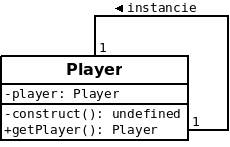
\includegraphics[scale=0.5]{Singleton.png}
    \caption{Diagramme UML du player implémentant le pattern Singleton}
  \end{center}
\end{figure}

\paragraph{Factory}

Le pattern Factory permet de déléguer la création des objets utiles à une classe tierce, afin de déporter ce type d'opération dans le code métier plutôt que dans le code client.

Dans le cas de cette application justement, il est apparu rapidement que le code client allait devenir lourd et répétitif, du fait des nombreux appels Ajax vers des APIs différentes. Il fallait donc trouver un moyen d'éviter la répétition ; ce que permettait dans un premier temps l'héritage. En créant une classe de requête spécifique pour chaque API et en faisant hériter tout cela d'une classe modèle (abstraite sans l'être vraiment), on gagne en flexibilité et on évite déjà beaucoup la redondance de code.

Cependant, il est apparu aussi bien vite qu'il n'était guère pratique de gérer l'instanciation de ces classes côté client. Il était alors judicieux d'ajouter une classe supplémentaire, la Factory, chargée de fournir la bonne instance de la bonne classe en fonction des paramètres passés à sa méthode de création (getAjaxRequest).

La méthode de création n'étant d'ailleurs pas statique, la Factory doit elle aussi être instanciée. Plusieurs instances de Factory peuvent alors cohabiter, mais ce n'est pas un impératif. Une seule instance de Factory peut très bien gérer plusieurs requêtes.

\begin{figure}[!h]
  \begin{center}
    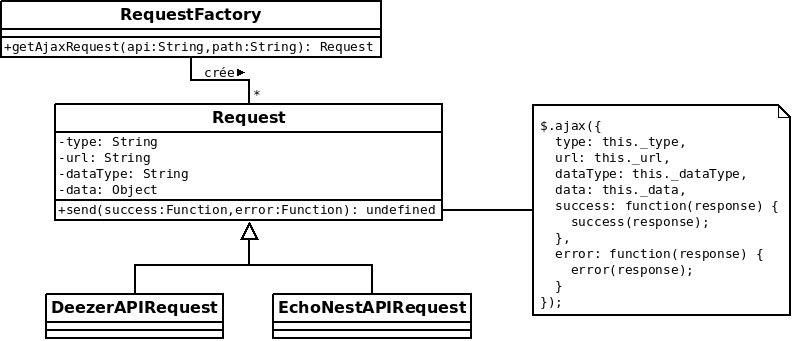
\includegraphics[scale=0.5]{Factory.png}
    \caption{Diagramme UML d'une Factory de requêtes Ajax}
  \end{center}
\end{figure}

\newpage

\subsubsection{Patterns structurels}

Les design patterns structurels interviennent lorsqu'il convient d'architecturer son application de manière spécifique, tout en représentant clairement la relation entre les différentes entités. De tels patterns ne sont pas forcément nécessaires dans des projets de faible envergure, mais ils deviennent un atout lorsque la complexité d'un système croît, ce qui requiert de fait une organisation plus stricte.

\paragraph{Façade}

Le pattern Façade est très utilisé en JavaScript. Il permet de masquer la complexité d'un ou plusieurs sous-systèmes, en encapsulant toute la logique dans une méthode.

L'objectif est bien sûr de simplifier l'utilisation d'un ensemble de fonctionnalités dans le code client. Ce pattern s'avère d'ailleurs indispensable pour limiter la redondance de code.

Pour illustrer le principe, on pourrait prendre l'exemple de la méthode «~alert~», au sein du package GUI du projet.

\newpage

\begin{lstlisting}
GUI = {
  ...
  alert: function(type, message, timer) {
    if (GUI.notifAllowed) {
      switch (type) {
	case "success":
	  return alertify.success(message, timer);
	  break;
	case "error":
	  return alertify.error(message, timer);
	  break;
	case "warning":
	  return alertify.warning(message, timer);
	  break;
	case "message":
	  return alertify.message(message, timer);
	  break;
      }
    }
  },
  ...
}
\end{lstlisting}

Cette méthode est une implémentation du pattern Façade en ce qu'elle fournit au code client un unique point d'entrée simplifié pour gérer les notifications.

Ici, le code client (app.js) n'a pas conscience qu'une bibliothèque de notifications (AlertifyJS) est utilisée par le module GUI. Il ne sait pas non plus qu'un test est effectué pour vérifier si les notifications sont bien actives. Tout ce qui importe au client, c'est d'afficher une notification à tel endroit.

Si GUI n'était pas une Façade, le code client serait moins cohérent et beaucoup plus répétitif car il faudrait alors appeler une méthode différente pour chaque type de notification (success, error, message) et à chaque fois tester le statut (actif/inactif) des notifications avant de les afficher ou non.

Un exemple éloquent du pattern Façade en JavaScript se retrouve notamment dans jQuery, au travers des méthodes \$.get et \$.post qui facilitent l'utilisation de \$.ajax.

\newpage

\paragraph{Adapter}

Lorsqu'on utilise une API ou un SDK, il arrive parfois que des interfaces soient incompatibles avec le code que l'on a soi-même développé. Ce cas de figure se présente souvent en Java. Et en JavaScript, en dépit du fait que la notion d'interface soit moins prégnante qu'en Java, le problème reste le même. C'est d'ailleurs une bonne pratique de développement que de s'abstraire d'un code extérieur en l'adaptant à ses propres besoins.

C'est précisément ce qui a été fait dans ce projet avec la mise en place d'un Adapter pour le lecteur audio fourni par le SDK de Deezer. Toutes nos méthodes font ici de la délégation vers celles de DZ.player.

On remarquera, au passage, que notre Adapter est aussi notre Singleton !

\vspace{10pt}

\begin{figure}[!h]
  \begin{center}
    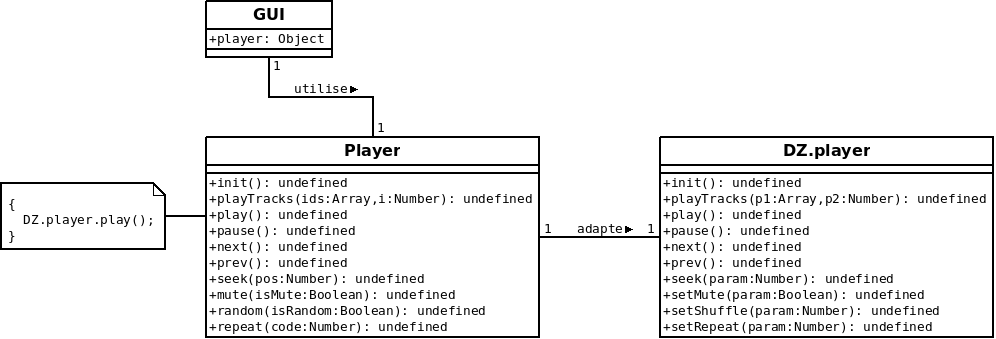
\includegraphics[scale=0.35]{Adapter.png}
    \caption{Diagramme UML d'un Adapter de lecteur audio (Deezer)}
  \end{center}
\end{figure}

\subsubsection{Patterns comportementaux}

Les design patterns comportementaux se focalisent sur la communication entre entités. Ils s'avèrent utiles pour flexibiliser et clarifier les interactions, directes et indirectes, entre les différents objets d'un programme.

\paragraph{Iterator}

En JavaScript, le pattern Iterator est beaucoup plus simple à mettre en œuvre qu'en Java. En Java, l'implémentation officielle du pattern Iterator est complexe et s'appuie également sur le pattern AbstractFactory. C'est tout le contraire en JavaScript où l'implémentation d'Iterator tient en une seule «~classe~».

Outre l'intérêt pédagogique de créer son propre itérateur, celui-ci s'avère utile dans notre application pour parcourir de façon plus agréable le tableau de morceaux généré à la fin de toutes les requêtes Ajax. Il faut néanmoins préciser que les implémentations d'Iterator ne manquent pas en JavaScript. Des bibliothèques comme jQuery ou Underscore.js font cela très bien avec leurs fonctions respectives \$.each et \_.each. Nativement, dans sa version 6 (cf. ECMAScript 6), JavaScript possède également une boucle for...of et un protocole itérateur qui remplissent exactement cet objectif.

\vspace{10pt}

\begin{figure}[!h]
  \begin{center}
    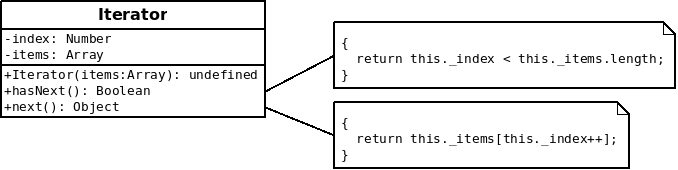
\includegraphics[scale=0.5]{Iterator.png}
    \caption{Diagramme UML d'un Iterator personnalisé}
  \end{center}
\end{figure}

\paragraph{Strategy}

Le pattern Strategy est utile lorsqu'il faut choisir, à l'exécution, entre plusieurs algorithmes effectuant différemment une même tâche. En JavaScript, du fait de l'inexistence des interfaces, l'implémentation de ce pattern varie quelque peu, mais les principes restent identiques.

Pour HARMONEEZER, Strategy s'est montré pertinent dans la mise en place d'un module de tri cohérent. Dans ce module, on retrouve notamment toutes les classes algorithmiques ainsi que la classe Strategy. Il est intéressant de noter que cette dernière possède un attribut représentant l'algorithme de tri courant et la méthode «~sort~» permettant de lancer le tri. À ce niveau, cette méthode est en quelque sorte abstraite et fait de la délégation vers la méthode «~sort~» de l'algorithme courant, déterminé côté client grâce à la méthode «~setAlgorithm~» de Strategy.

\begin{figure}[!h]
  \begin{center}
    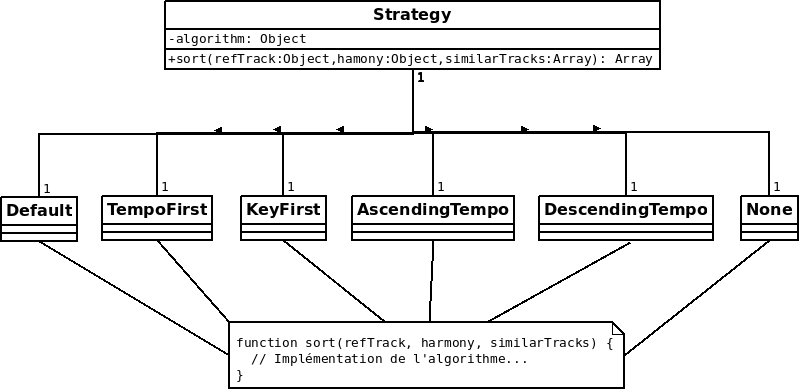
\includegraphics[scale=0.5]{Strategy.png}
    \caption{Diagramme UML d'une Strategy de tri}
  \end{center}
\end{figure}

\newpage

\subsubsection{Autres patterns}

Le monde des design patterns est riche et ne se limite pas à ceux énoncés par le GoF (Gang of Four). Nous allons ici voir les autres patterns qui se sont avérés très utiles pour ce projet ; en l'occurrence le pattern Module et le pattern MVVM.

\paragraph{Module}

D'après ce que nous avons dit plus haut, un programmeur JavaScript possède une très grande liberté. C'est à la fois un atout et une faiblesse du langage car il est fatalement possible de faire n'importe quoi et de mettre en œuvre une organisation bancale. En JavaScript, il existe cependant un pattern très important qu'il convient de suivre : le pattern \textbf{Module}.

Rappelons que JavaScript est avant tout un langage de script orienté prototype. Dans sa forme la plus classique, il n'y a donc aucune classe en JavaScript, contrairement par exemple à Java où même le point d'entrée du programme est forcément une classe.

\newpage

En JavaScript, reproduire le comportement d'une classe est déjà un design pattern. Ce pattern est connu sous le nom de «~Module~» car il permet de modulariser le code, et par extension de créer ses propres namespaces. Ceci est obtenu en encapsulant dans une fonction ou un objet un certain nombre de fonctionnalités. Cela passe notamment par l'utilisation de closures ou l'alimentation du prototype. Prenons un exemple simple...

Souvent, en JavaScript, on a un code qui ressemble à ça :

\begin{lstlisting}
function addition(a,b) { return a + b; }
function soustraction(a,b) { return a - b; }
function multiplication(a,b) { return a * b; }
function division(a,b) { return a / b; }
\end{lstlisting}

Toutes ces fonctions sont en général dans le scope global et sont appelées de la façon suivante :

\begin{lstlisting}
addition(1,2);
soustraction(3,1);
multiplication(1,3);
division(2,2);
\end{lstlisting}

Cette façon de procéder est problématique pour au moins deux raisons :

\begin{itemize}
 \item{Ces fonctions n'ont aucun lien entre elles, alors qu'elles servent un même objectif}
 \item{Cette architecture plate rend difficile la maintenance et les tests}
\end{itemize}

En suivant les principes de base du pattern Module, on a plutôt quelque chose qui ressemble à ça...

\begin{lstlisting}
var operation = {
  addition: function(a,b) { return a + b; },
  soustraction: function(a,b) { return a - b; },
  multiplication: function(a,b) { return a * b; },
  division: function(a,b) { return a / b; }
};
\end{lstlisting}

\newpage

... à ça ...

\begin{lstlisting}
function operation() {
  this.addition = function(a,b) { return a + b; };
  this.soustraction = function(a,b) { return a - b; };
  this.multiplication = function(a,b) { return a * b; };
  this.division = function(a,b) { return a / b; };
}
\end{lstlisting}

... à ça ...

\begin{lstlisting}
var operation = function() {}
operation.prototype.addition = function(a,b) { return a + b; };
operation.prototype.soustraction = function(a,b) { return a - b; };
operation.prototype.multiplication = function(a,b) { return a * b; };
operation.prototype.division = function(a,b) { return a / b; };
\end{lstlisting}

... ou encore à ça !

\begin{lstlisting}
var operation = function operation() {}
operation.prototype = {
  addition: function(a,b) { return a + b; },
  soustraction: function(a,b) { return a - b; },
  multiplication: function(a,b) { return a * b; },
  division: function(a,b) { return a / b; }
};
\end{lstlisting}

Les fonctions sont ensuite appelées de la façon suivante :

\begin{lstlisting}
var operation = new operation(); // Obligatoire SAUF dans le premier cas
operation.addition(1,2);
operation.soustaction(3,1);
operation.multiplication(1,3);
operation.division(2,2);
\end{lstlisting}

Une fois que toute la structure du module est prête, il ne reste plus qu'à l'exporter avec «~module.exports~». Browserify peut ensuite prendre le relais et encapsuler tout ça pour nous. À l'issue de la procédure, le module sera utilisable avec de simples «~require~» dans d'autres fichiers JS.

\begin{lstlisting}
module.exports = operation = {
  addition: function(a,b) { return a + b; },
  soustraction: function(a,b) { return a - b; },
  multiplication: function(a,b) { return a * b; },
  division: function(a,b) { return a / b; }
};
\end{lstlisting}

\paragraph{MVVM}

\begin{figure}[!h]
  \begin{center}
    
\includegraphics[scale=0.2]{logo-vuejs.png}
  \end{center}
\end{figure}

HARMONEEZER utilise Vue.js pour la création et la gestion des playlists. Alternative légère à AngularJS, Vue.js est un mini-framework permettant de mettre en place simplement le pattern MVVM dans une application, et ainsi de profiter de la puissance du data binding.

Le pattern MVVM (Model View ViewModel) est un cousin du pattern MVC (Model View Controller). Il permet de séparer clairement la logique métier du visuel, tout en conservant un lien fort entre les deux. Dans notre application, le modèle contient les morceaux qui ont été sélectionnés par l'utilisateur, tandis que la vue n'est rien d'autre que du HTML. L'instance de Vue, qui joue le rôle de ViewModel, nous permet de faire le lien entre notre modèle et notre vue. C'est notamment grâce à cette instance qu'une playlist peut être mise à jour. L'avantage d'une telle architecture, c'est que la vue reflète en temps réel l'évolution du modèle. Ainsi, dès lors qu'on ajoute ou qu'on supprime un morceau de la playlist, la vue se met immédiatement à jour.

Voici à quoi ressemble une instance de Vue permettant de gérer une liste d'éléments :

\newpage

\begin{lstlisting}
var vm = new Vue({
  el: "#app",
  data: {
    items: [
      { title: "Toto" },
      { title: "Tata" },
      { title: "Titi" }
    ]
  },
  methods: {
    addItem: function(item) {
      this.items.push(item);
    },
    removeItem: function(index) {
      this.items.splice(index, 1);
    }
  }
});
\end{lstlisting}

Pour afficher l'état de notre modèle dans notre vue, il nous suffit simplement d'itérer sur les items du modèle, en utilisant les directives fournies par Vue.js. Ceci a en quelque sorte pour effet de synchroniser notre vue et notre modèle. La syntaxe Mustache est utilisée pour le templating.

\vspace{7pt}

\begin{lstlisting}
 <ul>
  <li v-for="item in items">{{ item.title }}</li>
 </ul>
\end{lstlisting}

\subsection{Structure de l'application}

Si nous combinons maintenant tous les design patterns que nous venons d'expliciter, et que nous y ajoutons quelques classes garantissant le bon fonctionnement de l'application : nous aboutissons à un diagramme de classes fourni ; et pourtant nous sommes en JavaScript !

\textbf{N.B. Sur le diagramme UML, les constructeurs ainsi que les accesseurs ou mutateurs sont généralement implicites. C'est tout à fait volontaire, afin de ne pas trop surcharger l'ensemble.}

\begin{landscape}
  \begin{figure}
  \begin{center}
    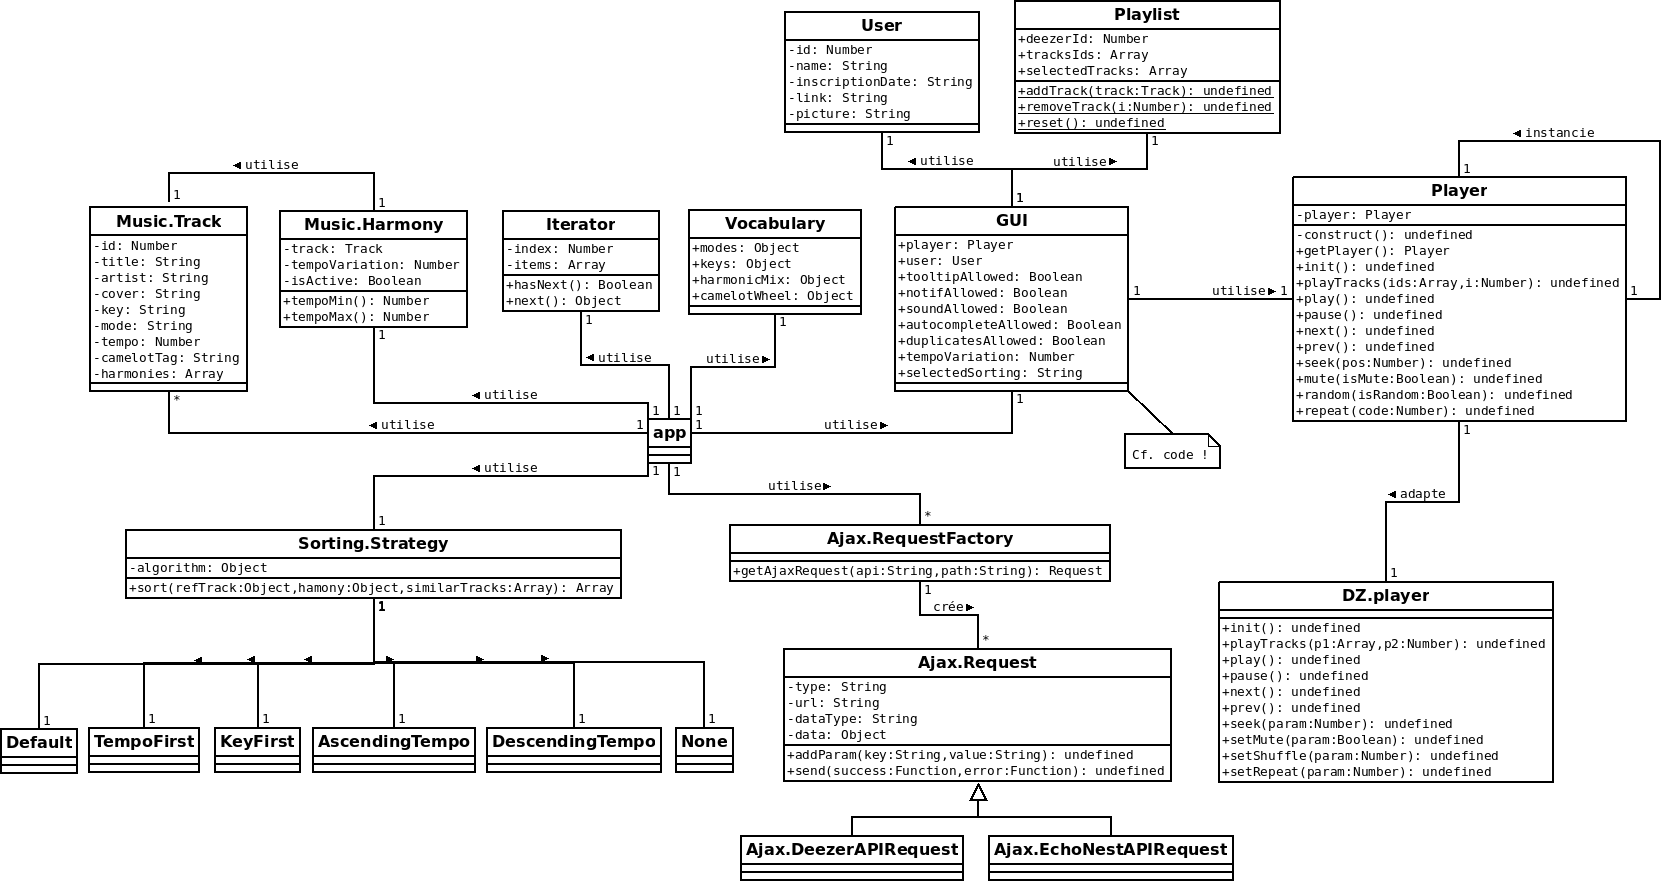
\includegraphics[scale=.4]{App.png}
  \end{center}
  \caption{Diagramme UML complet de l'application}
  \end{figure}
\end{landscape}

\subsection{Interrogation de deux APIs RESTful}

\begin{figure}[!h]
  \begin{center}
    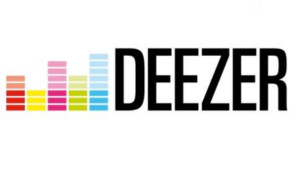
\includegraphics[scale=0.5]{logo-deezer.jpg}
    
\includegraphics[scale=0.5]{logo-echonest.png}
  \end{center}
\end{figure}

HARMONEEZER, en tant qu'application front-end, repose entièrement sur l'interrogation d'APIs (Application Programming Interfaces) en AJAX (Asynchronous JavaScript And XML). Autrement dit, toutes les données de l'application proviennent de serveurs distants appartenant à des sociétés tierces ; en l'occurrence Deezer et Spotify (Echo Nest).

Or, sur le Web, il y a une règle de sécurité importante connue sous le nom de «~same-origin policy~». Cette règle interdit explicitement les requêtes qualifiées de «~cross-domain~», ce qui signifie qu'il est normalement impossible d'interroger un domaine qui n'est pas de notre ressort.

Pour pallier ce problème, il existe deux types de solutions :

\begin{itemize}
 \item{JSONP (JavaScript Object Notation with Padding)}
 \item{CORS (Cross-Origin Resource Sharing)}
\end{itemize}

La différence entre ces deux techniques réside dans le fait que JSONP utilise une méthode de callback, tandis que CORS utilise des en-têtes HTTP spécifiques.

Dans le cadre de notre application, et bien que CORS soit techniquement plus «~propre~», c'est la méthode JSONP qui a été utilisée. En effet, l'API de Deezer, qui est au cœur de l'application, ne supporte pas CORS à l'heure actuelle. En tout cas, le format JSON a été privilégié pour sa simplicité d'utilisation en JavaScript, contrairement au XML... C'est d'ailleurs en JSON que la roue de Camelot a été traduite (manuellement) afin de permettre l'interaction avec les APIs !

Comme nous avons pu le voir précédemment dans ce rapport, les APIs de Deezer et Echo Nest ont principalement été interrogées à partir d'une Factory de requêtes Ajax. Mais ce que nous n'avons pas encore précisé, c'est le mode d'interrogation, avec son architecture sous-jacente... Ici, les APIs ont été interrogées conformément à l'architecture REST (REpresentational State Transfer), via des requêtes de type GET suivant une structure d'URL bien précise. Par exemple, pour récupérer les informations d'un morceau sur Deezer, il faut interroger cette URL en GET : http://api.deezer.com/track/\{id\}. Pour plus d'exemples, vous pouvez consulter l'\href{https://developers.deezer.com/api/explorer}{\textbf{API Explorer}} mis à disposition par Deezer afin de simuler des requêtes Ajax directement dans le navigateur.

Deezer et Echo Nest sont donc deux APIs agencées selon l'architecture REST. Le mode d'interrogation reste fatalement identique, mais chaque API a tout de même ses spécificités...

Si l'on se lance dans un rapide comparatif, du point de vue du développeur, l'API de Deezer est plus simple à utiliser et offre une plus grande liberté. Les données techniques telles que le tempo ou la tonalité y sont globalement moins précises, voire absentes, mais le développeur a un accès illimité et sans restriction à l'API.

Avec Echo Nest, la réalité est un peu différente car il faut renvoyer sa clé d'API à chaque requête, et de surcroît, il y a une limite assez embarrassante de 120 requêtes par minute (surtout quand on est contraint d'envoyer 50 requêtes par clic...). L'interaction entre Deezer et Echo Nest est une réussite car Echo Nest reconnaît de nombreux identifiants de morceaux Deezer. Cependant, à l'heure actuelle, les requêtes batch impliquant Deezer renvoient systématiquement une erreur 403 (Forbidden) sur Echo Nest, ce qui ne permet pas d'optimiser ses requêtes.

Enfin, dans le cadre de ce projet, certaines requêtes de type POST et DELETE sont également effectuées à l'aide du SDK fourni par Deezer. Par exemple, une requête POST est évidemment indispensable pour envoyer une playlist ou un morceau sur Deezer, et il en est de même pour une requête DELETE si l'on veut y supprimer des choses. L'intérêt du SDK pour ce type d'opérations est évident. On peut constater la simplicité d'utilisation de cet outil avec la requête suivante permettant de créer une playlist :

\vspace{7pt}

\begin{lstlisting}
DZ.api("user/me/playlists", "POST", {title : "Toto"}, function(response) {
  console.log("Identifiant de la playlist sur Deezer", response.id);
});
\end{lstlisting}

Ici on crée bien une playlist intitulée «~Toto~» sur le compte Deezer de l'utilisateur courant («~user/me~») !

\newpage

\subsection{Création d'interface graphique}

\begin{figure}[!h]
  \begin{center}
    
\includegraphics[scale=0.5]{logo-semanticui.png}
  \end{center}
\end{figure}

L'interface graphique de l'application s'appuie sur un framework peu connu mais offrant une alternative solide à Bootstrap ou Foundation : Semantic UI.

Semantic UI est un framework front-end complet constituant une base de travail pour tout ce qui a trait au trio HTML/CSS/JS. Il est doté d'un ensemble de classes CSS réutilisables, d'un catalogue d'icônes professionnelles, de grilles pour un design responsive, et de fonctions JavaScript facilitant la conception d'interfaces graphiques.

HARMONEEZER utilise Semantic UI comme simple support pour le visuel, ce qui signifie que le style des composants natifs du framework est généralement surchargé par la feuille de style principale de l'application. Cela explique notamment la présence fréquente de la règle «~!important~» dans notre feuille de style principale, justement pour écraser la configuration par défaut.

\subsection{Balisage sémantique avec métadonnées}

\begin{figure}[!h]
  \begin{center}
    
\includegraphics[scale=0.2]{logo-opengraph.png}
  \end{center}
\end{figure}


Depuis quelques années, on parle beaucoup de «~Web sémantique~» et de données structurées. L'idée est en quelque sorte de rendre le Web suffisamment porteur de sens pour que les machines elles-mêmes puissent comprendre, et non plus seulement lire et agréger, le contenu disponible. Pour ce faire, il faut avoir recours aux métadonnées qui vont venir enrichir le contenu de base, en apportant en quelque sorte de l'information sur l'information.

\newpage

HARMONEEZER utilise plusieurs types de métadonnées, listés ci-après :

\begin{itemize}
 \item{Le protocole Open Graph de Facebook}
 \item{Les Twitter Cards}
 \item{La spécification microdata, avec le vocabulaire de Schema.org}
\end{itemize}

Le principe de l'Open Graph et des Twitter Cards est simplement de fournir aux robots d'indexation des informations exploitables pour enrichir le partage de contenu. Il s'agit d'une certaine manière d'une extension des balises meta fournies nativement par le langage HTML. Exemple avec la célèbre «~meta description~»:

\vspace{7pt}

\begin{lstlisting}
<!-- Description native -->
<meta name="description" content="Lorem ipsum...">
<!-- Description Open Graph (Facebook) -->
<meta property="og:description" content="Lorem ipsum...">
<!-- Description Twitter Cards -->
<meta name="twitter:description" content="Lorem ipsum...">
\end{lstlisting}

Quant aux microdata, introduites par HTML5, il faut dire qu'elles s'avèrent particulièrement utiles pour donner du sens aux entités musicales manipulées par l'application. Grâce aux attributs fournis par la spécification (itemscope, itemtype, itemprop), et au vocabulaire disponible sur \href{http://schema.org/docs/full.html}{\textbf{Schema.org}}, il devient possible d'apporter un haut degré de précision au contenu. Exemple simple avec une composition musicale :

\vspace{7pt}

\begin{lstlisting}
<div itemscope itemtype="https://schema.org/MusicComposition">
  <span itemprop="name">Far Beyond The Sun</span>
  <span itemprop="composer">Yngwie Malmsteen</span>
</div>
\end{lstlisting}

Avec itemscope, on définit la portée de l'entité à définir. Avec itemtype, on précise le type d'entité concernée à partir du vocabulaire de Schema.org. Et enfin, avec itemprop, on énumère chaque caractéristique de l'entité, toujours à partir du vocabulaire de Schema.org.

\newpage

\subsection{Documentation des modules}

\begin{figure}[!h]
  \begin{center}
    
\includegraphics[scale=0.5]{logo-yuidoc.png}
  \end{center}
\end{figure}

En JavaScript, on a souvent tendance à négliger la documentation. Il faut dire qu'on utilise souvent ce langage pour créer de petits scripts côté client, par exemple pour gérer quelques animations qui apportent un peu de dynamisme à un site web.

Mais lorsqu'une application complète est développée avec JavaScript, il devient indispensable d'avoir une documentation claire pour que le code soit parfaitement explicite. Ceci est d'autant plus vrai lorsque le développeur s'aventure dans une conception modulaire avec de multiples classes et de nombreux fichiers (cf. pattern Module).

Pour ce faire, HARMONEEZER utilise le générateur de documentation fourni par la bibliothèque YUI (Yahoo! User Interface), soit YUIDoc. Très proche de Doxygen et de Javadoc dans son utilisation, YUIDoc permet de documenter le code de manière claire et précise à l'aide d'annotations.

Voici par exemple à quoi ressemble la documentation d'une méthode :

\vspace{7pt}

\begin{lstlisting}
/**
 * Fonction testant si un nombre est dans un tableau.
 *
 * @method inArray
 * @param {Number} nb Nombre
 * @param {Array} arr Tableau de nombres
 * @return {Boolean} Vrai si le nombre est dans le tableau, faux sinon
 */
 function inArray(nb, arr) {
   return (arr.indexOf(nb) > -1);
 }
\end{lstlisting}

\newpage

\subsection{Tests}

Tester son application est important si l'on souhaite vérifier que tout fonctionne comme prévu. Bien sûr, ces tests peuvent être manuels. Mais tout tester à la main est ardu, répétitif, et très fastidieux. En outre, des tests manuels peuvent difficilement être exhaustifs et ne permettent pas de mettre en avant les éventuelles régressions qu'on peut rencontrer en faisant évoluer le code. Il était donc raisonnable de faire des tests automatisés, à la fois unitaires et fonctionnels, mais aussi de performance.

\subsubsection{Tests unitaires}

\begin{figure}[!h]
  \begin{center}
    
\includegraphics[scale=0.7]{logo-qunit.png}
  \end{center}
\end{figure}

Les tests unitaires ont été réalisés à l'aide de QUnit, un outil développé par l'équipe à l'origine de jQuery. QUnit est un framework qui permet de tester du jQuery, mais aussi du JavaScript natif. Il s'appuie sur un petit catalogue de fonctions utiles pour les tests : equal, deepEqual, ok, notOk, throws, etc.

Voici la structure classique d'une fonction de test avec QUnit :

\vspace{7pt}

\begin{lstlisting}
QUnit.test( "Mon test unitaire", function( assert ) {
  assert.expect( 5 ); // Il y a 5 (autres) assertions dans mon scénario
  assert.equal(val, res, "==");
  assert.deepEqual(val, res, "===");
  assert.ok(val, "true");
  assert.notOk(val, "false");
  assert.throws( // On teste si une erreur est bien renvoyée
    function() {
      // Instructions susceptibles de renvoyer une erreur
    },
    Error,
    "Message d'erreur"
  );
});
\end{lstlisting}

Pour tester l'application avec QUnit, un dossier spécifique a été créé (cf. « test/unitTesting »). Ce dossier contient notamment un fichier HTML pour la visualisation des résultats, ainsi que le fichier de test proprement dit, contenant tout le code JavaScript avec les assertions.

Pour l'occasion, ce dossier possède aussi un bundle spécifique créé par Browserify, avec « tests.js » comme nouveau point d'entrée. Là encore, on voit tout l'intérêt du pattern Module et de Browserify... Avec ce type d'organisation, il est très facile de faire des tests module par module car tout est bien découpé. Sans cela, les tests auraient été bien plus compliqués.

Dans le cadre de cette application, les tests vérifient systématiquement les points importants qui pourraient poser problème en cas de régression. Par exemple, on vérifie bien que l'Iterator maison fonctionne comme prévu en testant chaque itération sur un tableau fictif.

On regarde aussi que l'héritage est bien effectué pour toutes les classes, en vérifiant par exemple qu'une requête Ajax renvoyée par RequestFactory est bien une instance de DeezerAPIRequest ou EchoNestAPIRequest, mais aussi une instance de Request.

On vérifie également que nos modules sont bien utilisés, en testant par exemple si une erreur est renvoyée lorsqu'on essaie d'appeler une classe comme une fonction standard, sans l'opérateur «~new~».

Enfin on vérifie que l'hydratation des objets se passe bien en testant les valeurs courantes de leurs attributs via leurs accesseurs.

Naturellement, tout n'a pas été testé. C'est impossible. En revanche, chaque module possède sa propre série d'assertions. C'est particulièrement utile pour s'assurer que chaque module a bien le comportement escompté, même si on n'est jamais vraiment à l'abri d'un bug...

\newpage

\subsubsection{Tests fonctionnels}

\begin{figure}[!h]
  \begin{center}
    
\includegraphics[scale=0.5]{logo-phantomjs.png}
    
\includegraphics[scale=0.5]{logo-casperjs.jpg}
  \end{center}
\end{figure}

Pour s'assurer que tout fonctionne comme prévu dans une application, les tests unitaires classiques ne sont pas suffisants. Ils doivent notamment être complétés par des tests fonctionnels vérifiant le bon comportement de l'application en fonction des actions de l'utilisateur. Là encore, il est tout à fait possible de faire ces tests à la main. Cependant, JavaScript étant par essence un langage événementiel, il est très pénible de répéter soi-même les mêmes opérations pour vérifier que tout fonctionne. Il est beaucoup plus simple de lancer une commande dans un terminal qui fait tout à notre place. C'est ce qui nous amène maintenant aux navigateurs virtuels (headless) tels que PhantomJS ou encore Zombie.js...

Pour ce projet, le choix s'est porté sur PhantomJS qui est un navigateur WebKit sans interface graphique, jouissant d'une certaine notoriété dans le milieu open source. PhantomJS a ici servi d'environnement d'exécution des tests fonctionnels. Dans le cas qui nous concerne, il a notamment été complété par CasperJS pour la mise en œuvre des scénarios.

CasperJS est en quelque sorte un outil qui se comporte comme un utilisateur lambda. Il effectue certaines actions dans un navigateur (en l'occurrence PhantomJS), et on peut vérifier en passant si ces actions correspondent bien à ce qu'on attend. Les comportements et les tests sont définis de façon programmatique dans un fichier JavaScript qui est lu par CasperJS.

À noter que CasperJS s'appuie sur les sélecteurs CSS, tout comme jQuery, pour cibler les éléments du DOM. Mais on peut tout à fait utiliser des expressions XPath en guise de sélecteurs, exactement comme avec Scrapy ; le framework Python pour la création de robots d'indexation.

Voici à quoi ressemble un scénario typique de test automatisé avec CasperJS et PhantomJS :

\newpage

\begin{lstlisting}
// On crée une rubrique de test (6 est le nombre d'assertions attendues)
casper.test.begin("Mon test fonctionnel", 6, function suite(test) {

    // On associe la série de tests à une URL spécifique
    casper.start("http://www.url.com", function() {
	// On vérifie que le titre de la page est correct
        test.assertTitle("Le titre de la page", "Titre OK");
        // On vérifie l'existence d'un élément du DOM
        test.assertExists("#container", "Existe");
        // On vérifie la visibilité d'un élément du DOM
        test.assertVisible("#container", "Visible");
        // On vérifie l'invisibilité d'un élément du DOM
        test.assertNotVisible("#container", "Invisible");
        // On remplit un champ de formulaire et on le soumet (true)
        this.fillSelectors("form", {
            "input[type='text']": "Mon texte"
        }, true);
        // On vérifie que le champ contient désormais la bonne valeur
        test.assertField("#monChamp", "Mon texte", "Champ OK");
	// On déclenche un clic sur un bouton
	this.click("#monBouton");
    });
    
    // On attend une seconde (CasperJS est très rapide...)
    casper.wait(1000).then(function() {
	// On vérifie si un nouvel élément a été ajouté au DOM
	test.assertEval(function() {
            return __utils__.findAll(".test").length > 0;
        }, "Ajout OK");
        // On redéfinit le viewport par défaut (400x300)
        this.viewport(1920, 1080);
        // On prend une capture d'écran du site à cet instant précis
        this.capture("screenshot.png");
    });
    
    // On lance réellement la suite de tests
    casper.run(function() {
	// On met fin au processus lorsque les tests sont terminés
        test.done();
    });
    
});
\end{lstlisting}

\subsubsection{Tests de performance}

\begin{figure}[!h]
  \begin{center}
    
\includegraphics[scale=0.2]{logo-benchmarkjs.png}
  \end{center}
\end{figure}

JavaScript est un langage puissant qui permet de réaliser des applications très avancées. Le problème, c'est que la puissance de ce langage se voit très rapidement limitée par la puissance du navigateur...

Lors du développement de notre application, le problème de la performance s'est posé plus d'une fois. Lorsque la quantité de code JavaScript est importante sur la même page, et que de nombreux scripts sont importés, le navigateur ne suit plus le rythme et l'application ne se comporte plus du tout comme prévu. Il est donc fondamental, en particulier pour les applications lourdes, d'effectuer des optimisations.

Pour HARMONEEZER, les optimisations mises en place sont les suivantes :

\begin{itemize}
 \item{Redondance de code évitée autant que possible}
 \item{Caching des longueurs de tableaux dans les boucles «~for~»}
 \item{Caching des sélecteurs jQuery utilisés fréquemment}
 \item{Valorisation des ids en guise de sélecteurs}
 \item{Utilisation de la fonction «~append~» en dehors des boucles}
 \item{Concaténation des bibliothèques externes (Bower)}
 \item{Packaging et minification du code (Browserify)}
 \item{Compression sans perte des images (Optimizilla)}
 \item{Utilisation de requêtes batch en Ajax}
\end{itemize}

Le bien-fondé de certaines de ces optimisations a ici été démontré par nos soins à l'aide de Benchmark.js, une bibliothèque JavaScript pour la réalisation de tests de performance.

Avec Benchmark.js, voici la structure classique d'une suite de tests comparatifs :

\newpage

\begin{lstlisting}
var suite = new Benchmark.Suite;

suite.on('start', function() {
  console.log('Lancement de la suite de tests...');
})
.add('test 1', function() {
  // Code à tester
})
.add('test 2', function() {
  // Code à tester
})
.on('cycle', function(event) {
  console.log(String(event.target));
})
.on('complete', function() {
  console.log('Le plus rapide est ' + this.filter('fastest').map('name'));
});
\end{lstlisting}

Dans le HTML, on peut alors mettre un écouteur d'événement sur un bouton et lancer la suite de test à partir du clic. De préférence, le test doit être asynchrone pour éviter de saturer le navigateur.

\vspace{7pt}

\begin{lstlisting}
<button onclick="suite.run({ 'async': true });">Test</button>
\end{lstlisting}

Pour le reste, cela relève de l'intuition... Il est évident que la minification du code et la compression des images réduisent la taille des ressources à charger, ce qui soulage forcément le navigateur. De même, il est évident qu'il est plus rapide de charger un gros fichier avec une seule requête HTTP qu'un bataillon de petits fichiers avec autant de requêtes vers le serveur !

Concernant les requêtes batch, il s'agit d'un mécanisme permettant de grouper les requêtes. C'est un point crucial d'optimisation pour une application qui s'appuie exclusivement sur des requêtes Ajax. Malheureusement, seules les requêtes batch de Deezer étaient ici exploitables. Celles d'Echo Nest ne permettaient pas de faire le lien avec les identifiants des morceaux sur Deezer...

\newpage

% ==========================================================================
% =============================== Conclusion ===============================
% ==========================================================================

\part*{Conclusion}

HARMONEEZER est une application web interactive qui s'inscrit résolument dans l'ère de la musique dématérialisée. Son objectif élémentaire est de fournir aux mélomanes et autres curieux les outils nécessaires à la recherche avancée de morceaux sur Internet, en fonction des goûts et des aspirations de chacun. Mais surtout, il s'agit là d'un assistant d'aide à la création de playlists harmoniques.

Construire des playlists est un exercice courant sur la Toile, mais pas avec cette dimension harmonique fondée sur la roue de Camelot. Pour mener à bien cette mission, HARMONEEZER utilise des données fiables fournies par deux poids lourds de la musique connectée : Deezer et Spotify (Echo Nest).

Entièrement réalisée en JavaScript, cette application front-end constitue indubitablement un exercice intéressant et un vrai approfondissement du langage. JavaScript possède un écosystème incroyablement riche et diversifié qui a passionné l'auteur de ces lignes, au même titre que le sujet lui-même.

Ce projet était d'ailleurs une occasion d'essayer enfin le développement JavaScript avec un angle d'attaque purement orienté objet. Il fallait prendre conscience de la puissance de ce modèle prototypal et de cette flexilité inhérente au langage qui offre un certain confort dans l'implémentation des différents design patterns.

Créez donc vos playlists harmoniques avec HARMONEEZER !

\newpage

\part*{Liens utiles}

\textbf{Contexte}

\begin{itemize}
 \item{\url{http://www.murielle-cahen.com/publications/p_deezer.asp}}
 \item{\url{https://fr.wikipedia.org/wiki/Crise_du_disque}}
 \item{\url{https://fr.wikipedia.org/wiki/Partage\_de\_fichiers\_en\_pair\_\%C3\%A0\_pair}}
\end{itemize}

\textbf{Mix harmonique}

\begin{itemize}
 \item{\url{http://www.mixedinkey.com/fr/Guide-Pratique}}
 \item{\url{http://fr.audiofanzine.com/bien-debuter/editorial/dossiers/demarrez-en-mix-harmonique-facilement.html}}
 \item{\url{http://www.andymacdoor.com/fr/blog/mix-harmonique-c6}}
 \item{\url{https://fr.wikipedia.org/wiki/\%C3\%89chelle\_chromatique}}
 \item{\url{https://fr.wikipedia.org/wiki/Cycle_des_quintes}}
 \item{\url{https://youtu.be/bASEJB4vAcE}}
\end{itemize}

\textbf{Bonnes pratiques}

\begin{itemize}
 \item{\url{https://learn.jquery.com/}}
 \item{\url{http://gregfranko.com/jquery-best-practices/#/}}
 \item{\url{http://lab.abhinayrathore.com/jquery-standards/}}
 \item{\url{http://www.crockford.com/javascript/javascript.html}}
 \item{\url{http://www.dofactory.com/javascript/design-patterns}}
 \item{\url{https://addyosmani.com/resources/essentialjsdesignpatterns/book/}}
\end{itemize}

\textbf{Documentation}

\begin{itemize}
 \item{\url{https://developers.deezer.com/api}}
 \item{\url{http://developer.echonest.com/docs/v4}}
 \item{\url{https://developer.mozilla.org/fr/docs/Web/JavaScript}}
 \item{\url{http://api.jquery.com/}}
 \item{\url{http://api.jqueryui.com/}}
 \item{\url{http://semantic-ui.com/}}
 \item{\url{http://sass-lang.com/documentation/file.SASS_REFERENCE.html}}
 \item{\url{http://browserify.org/}}
 \item{\url{http://gulpjs.com/}}
 \item{\url{https://git-scm.com/documentation}}
 \item{\url{http://underscorejs.org/}}
 \item{\url{https://vuejs.org/}}
 \item{\url{http://alertifyjs.com/}}
 \item{\url{http://yui.github.io/yuidoc/}}
 \item{\url{http://vegas.jaysalvat.com/documentation/settings/}}
 \item{\url{http://manos.malihu.gr/jquery-custom-content-scroller/}}
 \item{\url{http://api.qunitjs.com/}}
 \item{\url{http://docs.casperjs.org/en/latest/}}
 \item{\url{http://phantomjs.org/documentation/}}
 \item{\url{https://benchmarkjs.com/}}
 \item{\url{http://bower.io/docs/api/}}
 \item{\url{https://docs.npmjs.com/}}
 \item{\url{http://ogp.me/}}
 \item{\url{https://dev.twitter.com/cards/getting-started}}
 \item{\url{http://schema.org/}}
 \item{\url{http://www.owlcarousel.owlgraphic.com/docs/started-welcome.html}}
\end{itemize}

\textbf{Multimédia}

\begin{itemize}
 \item{\url{https://pixabay.com/fr/}}
 \item{\url{https://www.freesound.org/}}
\end{itemize}

\end{document}          
